\documentclass[12pt]{report}


\usepackage[catalan]{babel}
\usepackage[utf8]{inputenc}
\usepackage{graphicx}
\usepackage{wrapfig}
\usepackage{amsmath}
\usepackage{amssymb}
\usepackage{ragged2e} 
\usepackage{subfig}
\usepackage{caption}
\usepackage{subcaption}
\usepackage[usenames]{color}
\usepackage{xcolor}
\usepackage{float}
\usepackage{chngcntr}
\usepackage{ragged2e}
\usepackage{multirow}
\usepackage{vmargin}
\usepackage{hyperref}

\definecolor{naranja}{rgb}{1,0.5,0}
%\usepackage{natbib}
%\bibliographystyle{abbrvnat}

\title{Estudi de la Geometria Fractal en el pla Real i Complex}
\author{Gerard Lahuerta  i Valentí Torrents}
\date{Desembre 2019}

\setpapersize{A4}
\setmargins{3cm}       % margen izquierdo
{2.6cm}                % margen superior
{16.5cm}               % anchura del texto
{23.7cm}               % altura del texto
{10pt}                 % altura de los encabezados
{0cm}                  % espacio entre el texto y los encabezados
{0pt}                  % altura del pie de página
{1cm}                  % espacio entre el texto y el pie de página
\renewcommand{\baselinestretch}{1.5}

\begin{document}
\justifying
\maketitle


\newpage
\thispagestyle{empty}
\hspace{6cm}
    \begin{minipage}{0.5\linewidth}
        \vspace{10cm}%margen superior de minipage
        {\small
           Las nubes no son esferas, las montañas no son conos, las costas no son círculos, y las cortezas de los árboles no son lisas, ni los relámpagos viajan en una línea recta
        }
        \begin{flushright}
           \citeauthor{\textit{Benoît Mandelbrot (1969 -2)}}
        \end{flushright}
        \vspace{5pt}%margen inferior de la minipage
    \end{minipage}
 


\newpage
\setcounter{page}{3}
\pagestyle{plain}
\tableofcontents

\cleardoublepage
\addcontentsline{}{chapter}{}
\newpage

\centerline{\textbf{Resumen}}
 En este trabajo hemos hablado sobre fractales desde un punto más básico y sencillo hasta uno de más matemático y complejo. Para empezar, hemos tratado la definición de fractal y sus propiedades, junto con una breve explicación de la historia de estos. También hemos trabajado la relación que presentan estas figuras con el medio natural y nuestras vidas, hablando al mismo tiempo de las aplicaciones que estos pueden tener en diferentes ámbitos. A continuación, nos adentramos plenamente en nuestro trabajo, hablando, ahora si, de los fractales geométricos. Primero denominamos a los más conocidos y de los cuales hablamos en profundidad, describiéndolos, calculando sus propiedades y, en la mayoría de casos, programándolos en lenguaje C. Un punto importante del cual hablamos es el juego del caos, un estilo de iteración aleatoria que crea una figura sorprendente. Más adelante, empezamos a introducir los fractales complejos, los cuales tienen unas propiedades bastante diferentes de los previamente mencionados. Nos adentramos en algunos cálculos matemáticos necesarios para el entendimiento de los fractales complejos, como son las iteraciones de funciones complejas. Aun así, no profundizamos mucho en estos, puesto que habría acabado desviando la esencia del trabajo. Igualmente, tratamos sobre los conjuntos de Julia y de Mandelbrot, los cuales son visualmente espectaculares.



 \centerline{\textbf{Abstract}}
    In this project, we have talked about fractals from a more basic and simple point to a more mathematical and complex one. To begin with, we have discussed the definition of fractal and its properties, together with a brief explanation of their history. We have also worked on the relationship these figures present with the natural environment and our lives, while also talking about the applications that these can have in different areas. Next, we start to go deep into our project talking, now, about geometrical fractals. First we call the best-known ones, of which we speak in depth, describing them, calculating their properties and, in most cases, programming them in C language. An important point we talk about is the game of chaos, a style of random iteration that creates a surprising figure. Later on, we begin to introduce complex fractals, which have properties quite different from the previously mentioned ones. We get into some mathematical calculations necessary for the understanding of complex fractals, such as the iterations of complex functions. Despite that, we do not go deep into these, since it would have ended up diverting the essence of the work. 

\newpage
\chapter{Introducció}
\setcounter{page}{6 }
\section{Motivació i antecedents}
La realització d'aquest treball ha estat duta a terme per part de Gerard Lahuerta i Valentí Torrents, alumnes de Batxillerat a l'escola Sant Gervasi. En aquest Treball de recerca, hem volgut millorar els nostres coneixements envers els fractals, especialment els fractals geomètrics. Com és normal, en un principi no teniem gaire clar per quina branca de les ciències numèriques anar, ja que podiem optar per fer un treball de caire científic, o bé purament matemàtic. Definitivament, vam decantar-nos per fer un treball bassat purament en les matemàtiques i, després de fer recerca sobre diferents temes que ens podrien agradar, vam escollir el tema dels fractals. Sorprenentment, el món dels fractals és extremadament extens, pel qual haviem d'escollir una especialitat en la que centrar-nos. I aquesta va ser la geometria fractal. Vam escollir aquesta branca dels fractals ja que és la més vista al nostre dia a dia, amb organismes i invents formats a partir d'aquests.
\newline
En un principi no sabiem res sobre els fractals però, al parlar-ho entre nosaltres i amb el nostre tutor, l'interès va començar a creixer dins nostre. Un cop haviem decidit fer el treball sobre fractals, vam contactar amb la Universitat de Barcelona, on ens van comentar el tema amb molta més profunditat i ens van assessorar sobre com enfocar el treball. Allà ens van donar tot d'informació interessant amb la que vam entendre tot el necessari a saber sobre el món dels fractals.
\newline
Així, vam endinsar-nos en aquest treball amb moltes ganes i al·legria, treballant i estudiant d'una manera que mai haviem experimentat abans. En un principi no teniem uns objectius molt clars però és cert que hem assolit totes les nostres propostes i expectatives.
\newline
Al mateix temps, hem volgut fer una introducció molt extensa i fàcil d'entendre per tothom, ja que creiem que es tracta d'un tema molt interessant ja sigui acompanyat, o no, dels números i les matemàtiques que els caracteritzen.

\begin{itemize}
    \item \textbf{Investigacions prèvies}
\end{itemize}
Per tal d'iniciar aquest treball, vam haver de fer un estudi previ per tal d'entendre els fonaments dels fractals i la història dels mateixos. Més endevant parlem en profunditat dels estudis fractals al llarg de la història però, com a breu introducció, cal dir que els fractals han estat presents durant tota la història. En totes les èpoques hi ha hagut personatges que han treballat amb aquestes figures geomètriques que ningú entenia, i ha entès la seva utilitat.
\newline
En canvi, no va ser fins al 1997 que Benoît Mandelbort va emplear el terme fractal per primera vegada. Va se doncs, des d'aquell moment, que el món dels fractals ha evolucionat deixant un registre inmens d'aquest entre nosaltres.


\section{Objectius de la investigació }
Els nostres objectius a assolir al llarg d'aquest treball poden ser dividits en dues branques. En una podríem trobar els conceptuals i procedimentals, els quals es basen en la part pràctica del treball, i en l'altre podrem trobar els humans, que són els que permeten gaudir d'una adequada elaboració del treball.
\newline
Dins dels objectius conceptuals i procedimentals podem trobar:
\begin{itemize}
\item Ser capaços de fer un treball de recerca amb el rigor demanat, al mateix temps que poder exposar amb claredat el nostre treball final.
\item Aprendre a utilitzar LaTeX com a eina per a redactar treballs.
\item 


\end{itemize}
Ara, com a objectius humans trobariem:
\begin{itemize}
    \item Assolir un nivell de coneixements equitatiu entre tots els membres del grup, així com una cooperació adequada per complementar-nos mutuament.
    \item Coneixer experts en el tema per tal d'incrementar els nostres coneixements.
    \item Aprendre dels errors i adversitats que puguin sorgir al llarg del treball.
    \item Ser capaços d'escollir les millors opcions per tal de tirar endavant el treball, raonant cada problema des d'un punt de vista llògic.
\end{itemize}
\newpage
\section{Metodologia emprada}
Per a la creació d'aquest treball, hem utilitzat una gran varietat de recursos, des de TDR's d'alumnes d'anys anteriors de Sant Gervasi, fins a documents amb molta informació que hem trobat per internet. Al mateix temps, vam contactar amb la Universitat de Barcelona per saber si ens podrien fer la tutoria del treball. Afortunadament van accedir i, junt amb explicacions generals del tema, ens van entregar unes pautes a seguir per la redacció del treball i documents amb informació per al desenvolupament d'aquest. 
\newline
Com acabem de dir, ens vam posar en contacte amb la UB. Allà, la doctora Fagella, del departament de matemàtiques, ens va introduir el tema dels fractals, junt amb un estudiant de matemàtiques, David Balbuena, el qual ens faria la tutoria i ens assesoraria al llarg del treball. Allà, ens van donar documents per a l'entendiment i redacció de les parts més teòriques i matemàtiques, mentre que per la part històrica dels fractals vam haver de fer recerca pel nostre compte. 
\newline
Un altre dels aspectes en els que haviem d'ampliar els nostres coneixements va ser el de programar els fractals. Ja teniem una base per a la programació amb C++. Tot i així, la complexitat de les iteracions que haviem de dur a terme ens van obligar a buscar ajut en treballs relacionats o programacions similars, sortint-nos així endavant.
\newline
Per a la redacció del treball vam utilitzar un editor de textos especialitzat en textos científics anomenat LaTeX. Aquest ens ha permès introduir formules i caràcters matemàtics de forma més senzilla i ràpida. Tot i així, l'entendiment del funcionament d'aquest no ha estat del tot fàcil, pel que hem hagut de esforçar-nos en millorar les nostres habilitats utilitzant-lo.
\newpage
\chapter{Els fractals i la natura}
\section{Definició de fractal}
\justifying{
Per tal d'iniciar-nos en el món dels fractals, ens cal primer saber d'on prové la paraula i quin significat té.
\newline
El concepte de fractal prové de l'adjectiu llatí \textit{fractus}, que significa fracturat, trencat o irregular. Aquest concepte va ser primer desenvolupat per Benoit Mandelbrot, matemàtic polonès del Centre d'Investigació Thomas J. Watson dels laboratoris IBM a Nova York i pare de la geometria fractal, l'any 1975. Aquest terme els és atribuït a aquestes estructures perquè no poden ser considerades geomètriques com a tal, sinó com a semigeomètriques. 
Això és a causa de que no les podem establir representades explicitament en un pla o en una recta, sinó en un punt "mitjà" entre els dos.
\newline
D'altra banda, l'any 1975 Mandelbrot va afirmar que els fractals són formes generades normalment per processos matemàtics repetitius i caracteritzats per no ser diferenciables, per tenir un aspecte semblant a qualsevol escala i una dimensió fraccionària.
\newline
Al 1982 Mandelbrot va definir fractal com a un conjunt la dimensió del qual és estrictament major que la seva dimensió topològica, però ell mateix va reconèixer que aquesta última consideració no era suficientment general i excloïa alguns objectes matemàtics que realment són fractals com la corba de Peano. Tot i que continúa sent la definició més acceptada pels sectors matemàtics, al ser la més adequada per englobar figures fractals.
\newline
Mandelbrot no va inventar els fractals, sinó que va aconseguir agrupar i identificar certes propietats en comú entre aquestes construccions geomètriques anteriorment anomenades "monstres matemàtics", ja que sempre havien estat a la natura i als
límits de l'infinit a esperant que algú topés amb ells i donés a conèixer aquesta meravella matemàtica i artística.
\newline
La definició de fractal ha anat evolucionant amb el temps segons les característiques i propietats dels que s'anaven descobrint. El mateix Mandelbrot afirma que només disposem d'una definició temporal i incompleta, donat que cap definició teòrica resulta totalment satisfactòria. }

\section{Propietats fonamentals}
Primer de tot, cal recordar que Mandelbrot no va donar una definició precisa de fractal però de forma general va caracteritzar les noves estructures irregulars com figures autosimilars, de complexitat infinita, de dimensió fraccionària i recursives.
\newline
A partir d'aquesta caracterització, podem parlar sobre algunes de les propietats més importants dels fractals en general.

\begin{itemize}
\item \textbf{Autosemblança o autosimilitud:}
\end{itemize}

\begin{wrapfigure} {l} {0.25\textwidth}
%\centering
    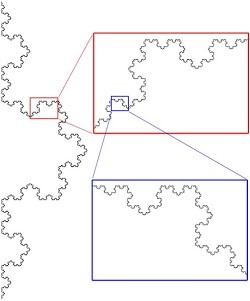
\includegraphics [width=0.25\textwidth] {foto.jpg}
    \caption{Exemple d'autosemblança}
\end{wrapfigure}

La autosemblança és un concepte que es pot entendre de manera simple i bastant visual. Imaginem un objecte geomètric, indiferentment de la forma que tingui. Ara, pensem que aquest objecte o figura està format per figures idèntiques a l'original, però amb una mida reduïda; i alhora cadascuna d'aquestes figures està composta per unes de més petites que se segueixen veient idèntiques a l'original, així successivament... Entenent aquest procediment, podem tenir una imatge clara de com pot arribar a ser qualsevol fractal.
\newline
Aquesta característica rep aquest nom a causa de que totes les figures que formen el nostre objecte són semblants a l'original, sabent que dues figures són semblants entre elles si tenen la mateixa forma però diferents mides.
\newline
\newline
\newline
\begin{itemize}
\item \textbf{Recursivitat:}
\end{itemize}

\begin{wrapfigure} {l} {0.25\textwidth}
%\centering
    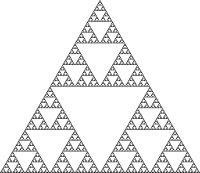
\includegraphics [width=0.2\textwidth] {recursivitat.png}
    \caption{Triangle de Sierpisnki}
\end{wrapfigure}
Aquesta característica és pròpia dels fractals, ja que es tracta de conjunts definits per un algoritme recursiu amb processos iteratius determinats. Això vol dir que poden ser formats repetint el mateix procés infinites vegades.
El procés, del qual parlarem més a fons més endavant, es tracta d'aplicar una iteració a una figura inicial, i seguir aplicant la mateixa iteració al resultat obtingut al aplicar-la anteriorment.
\newline

Gràcies a aquesta qualitat, els fractals possibles de programar amb ordinador a partir de, com ja hem dit, un algoritme recursiu repetit una infinitat de vegades.

\begin{itemize}
    \item \textbf{Complexitat infinita}
\end{itemize}
Aquesta característica ens indica que, indiferentment de l'escala d'observació amb la qual la veiem, la figura sempre manté molta complexitat.
\newline
Gràcies a aquesta propietat, podríem ampliar una imatge sense parar i la figura que se'ns mostraria seria totalment idèntica a la inicial.
\newline
El fet que els fractals tinguin una bellesa peculiar és producte d'aquesta complexitat infinita que, al no ser extremadament complicada d'imaginar o detectar en una figura, és més atractiva per les persones que ho veuen.
\newline
\newline
La manera més simple i eficient de classificar fractals és fer-ho en funció de les característiques que acabem d'anomenar. Així i tot, aquesta classificació, com qualsevol altre, ens porta a deixar de banda altres característiques que podrien relacionar o diferenciar més aquestes figures.
\newline
A trets generals, parlem de dos grups ben diferenciats i definits depenent de si s'iteren en reals o en complexos, termes dels quals parlarem més endavant:
\newline
\newline
-\textbf{Fractals lineals:} aquests poden ser construïts a partir d'un senzill canvi en les seves escales. A causa d'aquesta propietat, tenen exactament la mateixa forma independentment de l'escala fins a l'infinit en la que es trobi. Alguns exemples serien el triangle de Sierpinski o la corba de Koch.
\newline
\newline
-\textbf{Fractals no lineals:} són aquells que es generen a partir de distorsions complexes o no lineals. La
majoria dels objectes fractals purament matemàtics i naturals no són lineals, com el conjunt de
Mandelbrot o el conjunt de Julia.

\section{Fractals a la natura}
Ara que ja ens hem endinsat una mica en el complex món dels fractals, i abans d'aprofundir en l'aspecte matemàtic d'aquests, és bastant oportú que tractem la seva importància i abundància a la naturalesa que ens envolta. A continuació, parlarem d'alguns exemples de fractals que podem arribar a trobar a qualsevol paisatge. Ens haurem de fixar, també, en com compleixen les característiques anteriorment mostrades.
\newline
Des de ben petits, tots hem expressat la realitat d'una manera molt simple i geomètricament poc complicada, dibuixant-ho tot molt poc detallat i inexacte. Això és a causa del fet que la geometria euclidiana ho ha simplificat tot molt, fent que representéssim tot amb rectes, corbes o punts poc exactes i complexos. Ara bé, tots sabem que la realitat és extremadament diferent, ja que totes les figures que podem veure són extraordinàriament complexos, si saps a quina escala mirar. D'això tracta el llibre de Benoît Mandelbrot, \textit{Geometria Fractal de la Naturalesa.}
\newline
\begin{wrapfigure}{r}{0.35\textwidth}
    %\centering
    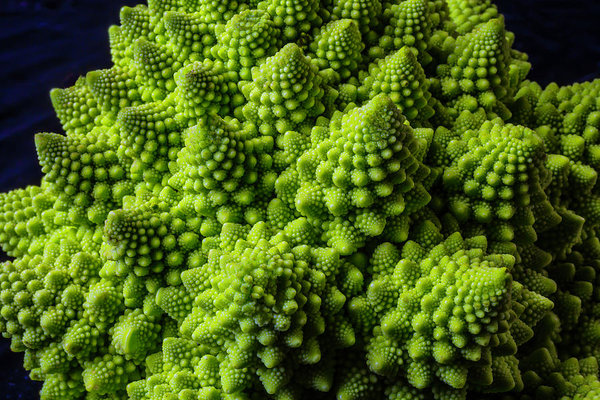
\includegraphics[width=0.33\textwidth]{romanesco.jpg}
    \caption{Romanesco}
    \end{wrapfigure}
Quan diem que la geometria fractal està present a la natura, no volem dir que sigui fàcil de detectar o que sigui visible a ull nu. Tal com hem dit abans, el que més importa per detectar aquests fractals a la naturalesa és variar el punt de vista i l'escala amb la qual els observem normalment. Per això, anem a anomenar alguns exemples de figures fractals presents als paisatges que podem haver vist.
\newline
\newline
\newline
La majoria de la gent no té una gran estima per les verdures o pels productes que ens otorga la terra però, més enllà del gust que puguin tenir, moltes d'elles mostren una geometria formidable, especialment la família de les cols. El més evident i espectacular fractal vist en un aliment d'aquest grup és el romanesco, el qual presenta una autosimilitud gairebé exacte.
\newline
\newline
Un altre exemple curiós pot ser la falguera, una de les primeres plantes en aparèixer al nostre planeta. La forma de les seves fulles és molt peculiar, però el valor estètic no és el més important per la planta a l'hora de crear les seves fulles així. Aquesta forma i distribució de les fulles compleix amb algunes de les característiques pròpies dels fractals, el que fa que puguin ocupar una major superfície per tal de captar el màxim de llum, $CO_2$ i oxigen.

\begin{wrapfigure} {l} {0.25\textwidth}
%\centering
    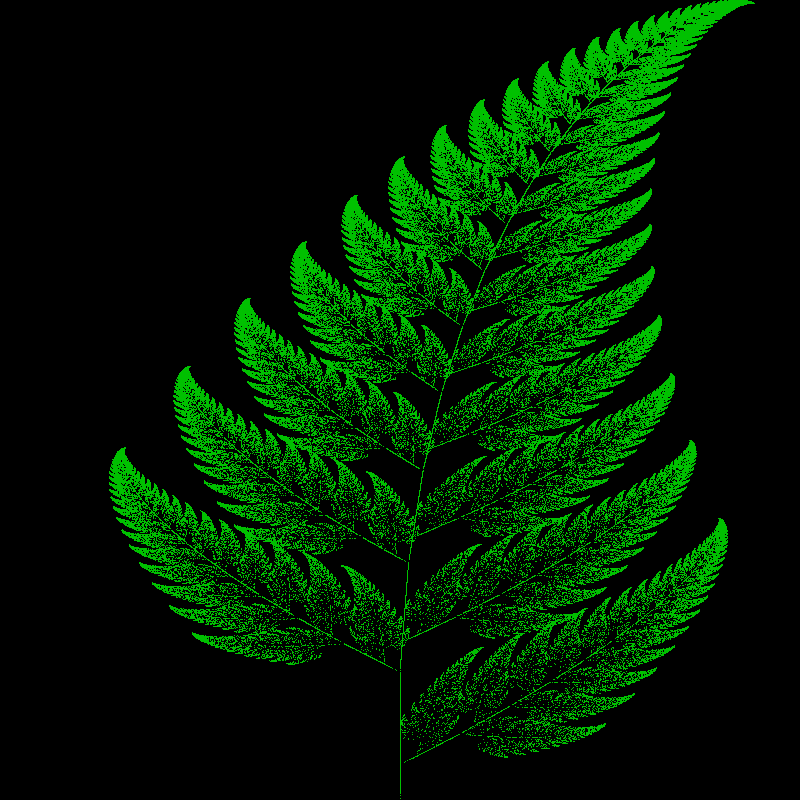
\includegraphics [width=0.20\textwidth] {fractal.jpg}
    \caption{Ramificacions fractals}
\end{wrapfigure}

A causa d'aquesta eficàcia i a la senzillesa amb la qual aquestes bifurcacions de les branques són creades, el disseny de la falguera o similars són dels més abundants a la natura. Aquestes ramificacions poden ser considerades fractals, però no de complets, ja que, al ser creats naturalment, han de tenir un nombre finit d'iteracions. Aquest tipus de fractals creats biològicament són els anomenats "fractals naturals".
\newline


\begin{wrapfigure}{r}{0.3\textwidth}
    %\centering
    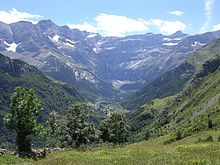
\includegraphics[width=0.3\textwidth]{muntanya.jpg}
    \caption{Paissatge muntanyós}
    \end{wrapfigure}
Un altre exemple evident de fractals visibles a la natura pot ser el perfil d'una muntanya. Aquest és constantment modificat pel vent, l'erosió, i molts altres factors. A diferència dels fractals naturals dels quals hem parlat abans, aquest no presenta una estructura idèntica en tots els seus punts.
En canvi, no som capaços de diferenciar cap dels seus punts, ja que mantenen una estructura molt similar, encara que no idèntica. Això també passaria al comparar el perfil de qualsevol serralada amb el d'una pedra vista de ben a prop.
\newline

\begin{wrapfigure}{l}{0.49\textwidth}
    %\centering
    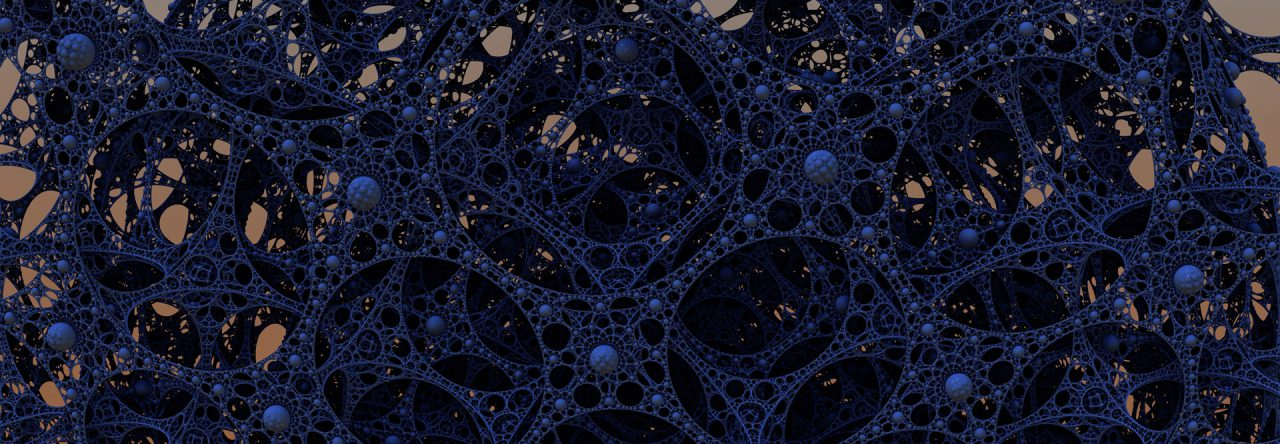
\includegraphics[width=0.5\textwidth]{fractalcuerpo.jpg}
    \caption{Interior del cos humà}
    \end{wrapfigure}
Per seguir donant exemples de fractals visibles en el nostre món, haurem de deixar de mirar fora per començar a mirar dins nostre. Algunes de les estructures fractals més impressionants es troben dins el nostre organisme i, sorprenentment, tenen molt avantatge. Al tenir les venes o artèries estructurades amb un disseny molt similar al dels fractals, ens permet cobrir el màxim de cèl·lules possibles per tal d'alimentar-les apropiadament. En el cas dels bronquis i els alvèols pulmonars, ens permet aprofitar el màxim cada inspiració i expiració per tal d'intercanviar més oxigen i diòxid de carboni. I no es queda aquí. Aquest estil d'estructura es troba a molts altres punts del nostre cos; com en el sistema sanguini, limfàtic, digestiu, pulmonar, o en les neurones i sistema nerviós; i otorga en totes elles un millor funcionament.
\newline
A continuació, mostrarem alguns més exemples de fractals visibles a la naturalesa. Cal recalcar que aquests són figures fractals més conegudes o amb menys utilitats, motiu pel qual els donem menys importància i no els descriurem un per un.
\newline

    
    \begin{figure} [H]
 %\centering
  \subfloat{
    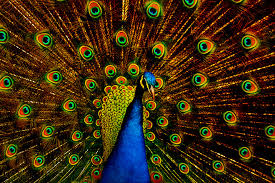
\includegraphics[width=0.34\textwidth]{pavo.jpg}}
  \subfloat{
    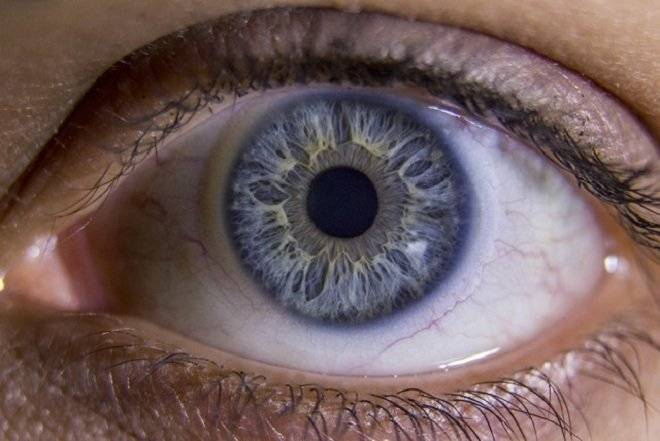
\includegraphics[width=0.34\textwidth]{ojo.jpg}}
  \subfloat{
    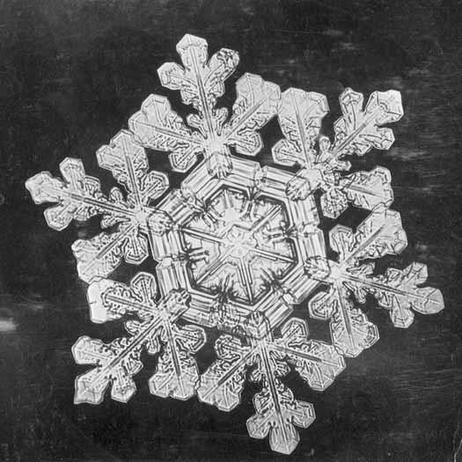
\includegraphics[width=0.23\textwidth]{snowflake.jpeg}}
\end{figure}
  \begin{figure} [H]
% \centering
  \subfloat{
    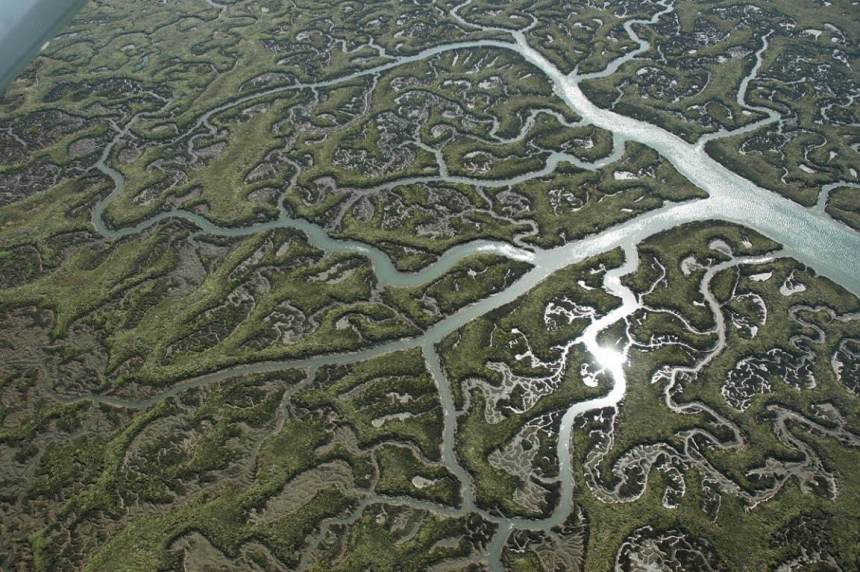
\includegraphics[width=0.38\textwidth]{6.jpg}}
  \subfloat{
    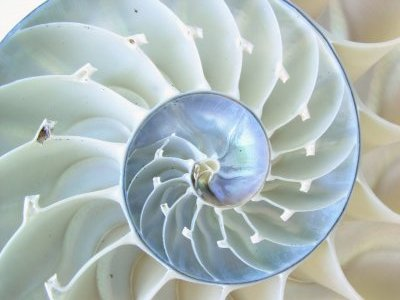
\includegraphics[width=0.34\textwidth]{nautilus.jpg}}
    \caption{Exemples de fractals a la natura}
\end{figure}
    
\newpage
\section{Aplicacions}
Un altre dubte que li sorgeix a tothom quan comencen ha sentit parlar sobre fractals és: \textit{quina utilitat tenen?} Doncs moltes, i en una gran varietat d'àmbits, algun dels quals potser ens toca estudiar o practicar en algun punt de les nostres vides, depenent dels estudis que fem.
\newline
A continuació, parlarem una mica sobre les utilitats que tenen els fractals en diversos àmbits com la tecnologia, la ciència, la biologia o l'art.
\subsection{Fractals a la ciència}
Òbviament, el primer que se'ns ve al cap quan escoltem sobre fractals és relacionar-ho amb la ciència o les matemàtiques, encara que no sapiguem ben bé com són aplicats. Doncs, sorprenentment per a molts, en té moltes d'aplicacions.
\newline
\begin{wrapfigure}{r}{0.3\textwidth}
    %\centering
    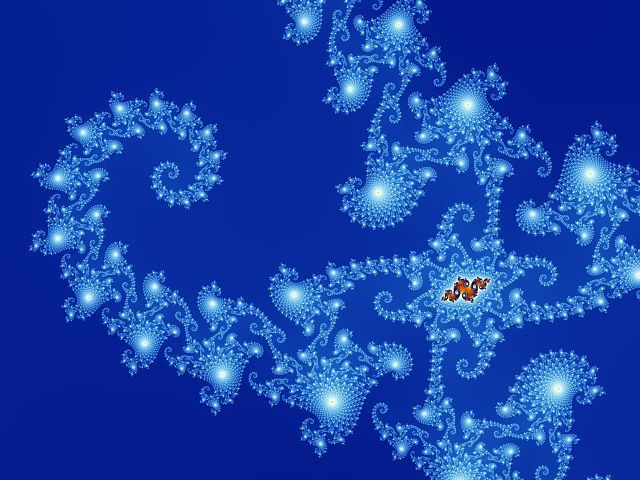
\includegraphics[width=0.3\textwidth]{ciencia.jpg}
    \caption{Fractal complex}
    \end{wrapfigure}
Primerament, cal parlar de la seva importància a les matemàtiques, i en la geometria. Podríem parlar de la teoria del caos per establir processos aleatoris o del mètode de Newton per aproximar arrels.
\newline
A continuació, podríem tenir en compte les seves aportacions a la física. Potser la seva importància no destaca per les seves aplicacions a la física teòrica, però en àmbits com la meteorologia es tornen sorprenentment importants. També podem observar aplicacions dels fractals en aspectes militars, com per exemple l'estudi de la variació en el comportament de les naus davant el vent.
\newline
I, per descomptat, també els trobem rellevants a la química i la biologia, on se li dóna una gran importància a la seva geometria a l'hora de fer compostos amb propietats peculiars o al estudiar plantes amb formes fractals.
\newline
\newline
\newline
\subsection{Fractals a la tecnologia}
\begin{wrapfigure}{l}{0.3\textwidth}
    %\centering
    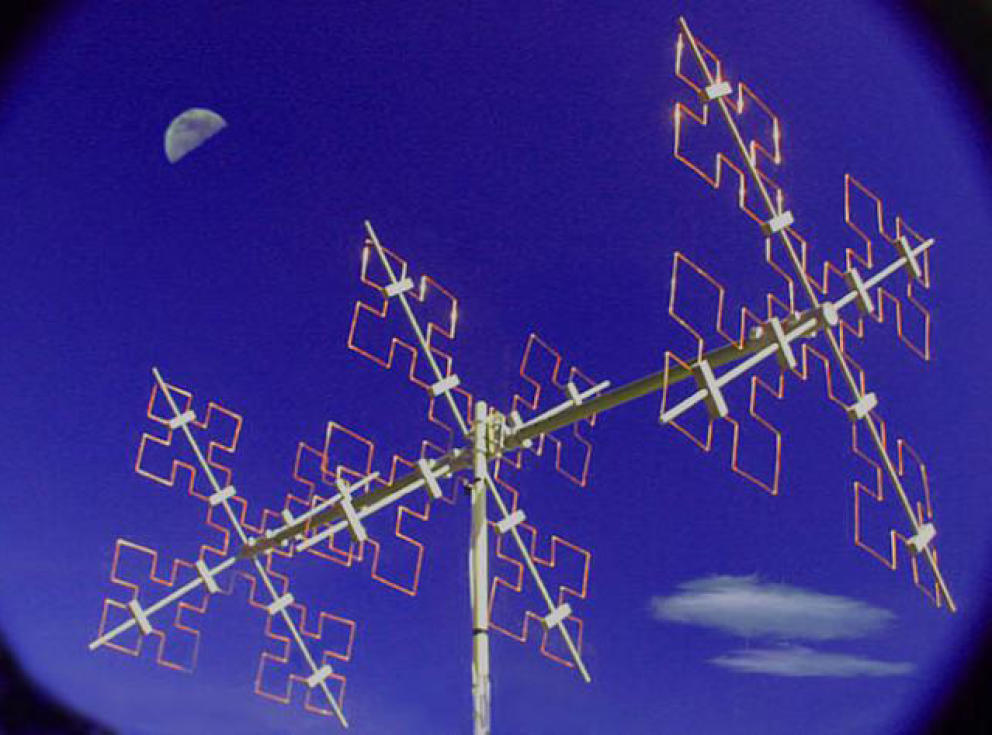
\includegraphics[width=0.3\textwidth]{antena.jpg}
    \caption{Tecnologia fractal}
    \end{wrapfigure}
En el món de la tecnologia, els experts sempre han intentat treure bon profit als fractals, tant en la codificació de senyals d'àudio, vídeo o digital, així com la compressió d'imatges. Una de les aplicacions principals es tracta de buscar algoritmes recursius similars als utilitzats per a la construcció dels fractals per tal de guardar la fórmula que genera una part de la imatge en lloc d'una porció d'imatges d'ella mateixa, reduint la memòria necessària.
Però l'aplicació més exitosa i enginyosa són les antenes fractals perquè han permès disminuir la seva grandària i el seu rendiment gràcies a aplicar les propietats fractals en
dispositius mòbils, com l'empresa catalana "Fractus S.A." amb gran influència internacional per aquesta brillant idea. 

\subsection{Fractals al art}


\begin{wrapfigure}{l}{0.4\textwidth}
    %\centering
    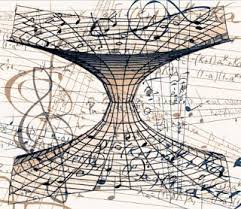
\includegraphics[width=0.4\textwidth]{musica.jpg}
     \caption{Fractals a la música}
    \end{wrapfigure}Veure pintures o escultures formades per figures fractals pot ser relativament fàcil, ja que només es tracta de representar, no a la perfecció, la geometria que hi ha darrere d'aquestes figures matemàtiques. Encara i així, hi ha altres estils d'art on no és tan senzill representar-les. Un exemple d'aquests és la música, on la versió fractal d'aquesta és bastant diferent de les vistes fins ara. La música fractal consisteix, principalment, en la projecció de l'estructura d'un fractal sobre un espai musical per generar composicions interessants.
Seria bastant improbable detectar una composició de música fractal sense tenir un nivell avançat en aquest aspecte. Però, un cop pots comprendre el rerefons darrere la música, podràs quedar molt sorprès per aquestes peces musicals.
    \newpage
    
 

\section{Dimensió fractal}
Com hem mencionat en la introducció, fractal significa fracturat o trencat i això és a causa de que no pertanyen a les dimensions a les que estem habituats (dimensió 0 un punt, 1ª dimensió una recta ...) sinó que per a definir-les necessitem dimensions fraccionàries.
\newline
Segons Mandelbrot i la seva definició de fractal, un fractal és aquell que la seva dimensió és estrictament major a la seva dimensió topològica. Per tant, per a definir i calcular les dimensions de qualsevol fractal, abans hem de definir què és la dimensió Topològica.
\begin{itemize}
\item \textbf{Dimensió Topològica:}
\end{itemize}

    
El concepte de dimensió Topològica habitual és el d'aquella dimensió que ve donada per un nombre natural. Però, hi ha altres definicions per al concepte de dimensió topològica. Una d'elles és la següent:

\begin{wrapfigure}{r}{0.4\textwidth}
   % \centering
    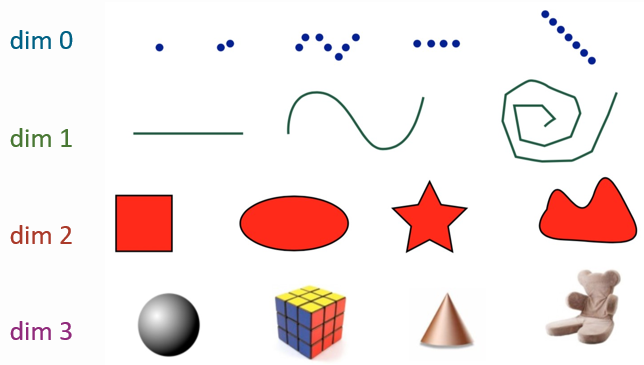
\includegraphics[width=0.4\textwidth]{Dim.PNG}
    \caption{Ambdues figures, adalt i abaix, representen les dimensions topològiques.}
    \end{wrapfigure}
\textcolor{red}{Definició} Sigui $S$ un subconjunt de $\mathbb{R}^N$ 
\begin{itemize}
\item [$-$] \textcolor{red}{$S$ té dimensió zero}, si cada punt té arbitràriament altres punts al voltant que, a la vegada, no intercepten entre ells.
\end{itemize}
\begin{itemize}
\item [$-$] \textcolor{red}{$S$ te dimensió $k$}, si el límit de cada punt de $S$ intercepta $S$ en un conjunt de dimensions $k-1$, on $k$ és el menor nombre natural per al qual l'anteriorment dit, succeeix.
\newline
\newline
\end{itemize}

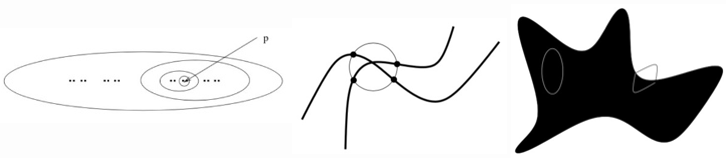
\includegraphics[width=0.8\textwidth]{Top.PNG}
\newline
\newline
\newline
\hspace*{4.5em}Dimensió 0 \hspace*{7.5em} Dimensió 1 \hspace*{7em} Dimensió 2
\newline
\newline
També podem relacionar la dimensió topològica com l'exponent que relaciona el nombre de peces en que pots dividir un objecte geomètric amb la seva contracció tal com ho explicarem en la pàgina següent.
\newline
Però, per a descriure la dimensió d'un fractal, necessitem una nova moció (o dimensió) per a mesurar la seva complexitat, ja que la descripció actual de la dimensió topològica no distingeix correctament els diferents tipus de fractals així com les seves densitats.
\begin{itemize}
\item \textbf{Com calcular la dimensió d'un fractal}
\end{itemize}
La fórmula per la qual puguem calcular la dimensió de qualsevol fractal també ha de ser vàlida per a les figures geomètriques (les que la seva dimensió sigui definida mitjançant un nombre natural).
\newline Per començar, agafarem el concepte d'autosimilitud de la geometria fractal amb fractals que tinguin el mateix factor de contracció en totes les seves afinitats per tal de trobar una aproximació a la fórmula per després depurar-la fins a trobar-ne una que sigui funcional.

\begin{wrapfigure}{l}{0.6\textwidth}
   % \centering
    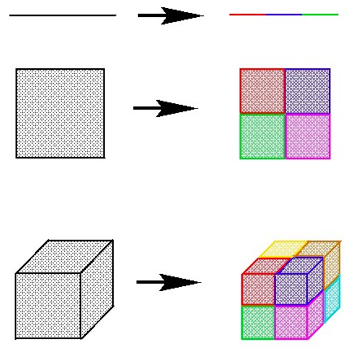
\includegraphics[width=0.6\textwidth]{Relacion-pieza-Dimension.PNG}
    \caption{Contraccions}
    \end{wrapfigure}

 \hspace*{0.5em}\begin{tabular}[t]{|c |c |}
\hline
Peces 3 & Contració: 1/3\\
\hline
Peces $J$ & Contració: 1/J\\
\hline
\end{tabular}      
\newline
      \newline
      
 \hspace*{0.5em}\begin{tabular}[t]{|c |c |}       
\hline
Peces 4 & Contració: 1/2\\
\hline
Peces $J^2$ & Contració: 1/J\\
\hline
\end{tabular}       
\newline
\newline
\newline
      
 \hspace*{0.5em}\begin{tabular}[t]{|c |c |}       
\hline
Peces 8 & Contració: 1/2\\
\hline
Peces $J^3$ & Contració: 1/J\\
\hline
\end{tabular}    
\newline 
\newline
\newline 
\newline
\newline
\newline 
\newline 
\begin{figure}
Podem observar que existeix una relació entre el nombre de peces, la contracció i la dimensió de les figures anteriors. 
\newline
Sent: $N$ el nombre de peces, $R$ el valor de la contracció i $D_S$ la dimensió d'un objecte $S$, trobem la següent expressió.
\end{figure}
\newline
$$N= {\left( \frac{1}{R} \right)}^{D_S} \Rightarrow D_S = \frac{ \log{(N)}}{\log{(\frac{1}{R}})}$$
Comprovem si la expressió trobada és correcte mitjanzant les taules anteriors.
\newline
Si $s$ és una línia $\longrightarrow$ $D_S = \frac{ \log{N}}{\log{\frac{1}{\frac{1}{N}}}} = \frac{\log{N}}{\log{N}} = 1$
\newline
Si $s$ és un quadrat $\longrightarrow$ $D_S = \frac{ \log{N^2}}{\log{\frac{1}{\frac{1}{N}}}} = \frac{\log{N^2}}{\log{N}} = 2$
\newline
Si $s$ és un cub $\longrightarrow$ $D_S = \frac{ \log{N^3}}{\log{\frac{1}{\frac{1}{N}}}} = \frac{\log{N^3}}{\log{N}} = 3$
\newline
Ara apliquem aquesta fórmula a fractals geomètrics que tinguin el mateix factor de contracció, així com el triangle de Sierpinski o la curva de Koch.
\newline

\begin{wrapfigure}{l}{0.2\textwidth}
    %\centering
    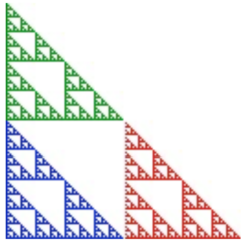
\includegraphics[width=0.2\textwidth]{DimS.PNG}
    \caption{Dimensió sierpinski}
    \end{wrapfigure}
$$D_{Sierpinski} = \frac{ \log{N_S}}{\log{\frac{1}{\frac{1}{R_s}}}}= \frac{ \log{3}}{\log{\frac{1}{\frac{1}{2}}}}= \frac{\log{3}}{\log{2}} = 1.58 ...$$
\newline
\newline
\newline
\newline
\newline

\begin{wrapfigure}{l}{0.2\textwidth}
    %\centering
    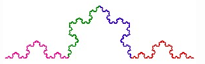
\includegraphics[width=0.2\textwidth]{DimK.PNG}
    \caption{Dimensió Koch}
    \end{wrapfigure}
$$D_{Koch} = \frac{ \log{N_K}}{\log{\frac{1}{\frac{1}{R_k}}}} = \frac{ \log{4}}{\log{\frac{1}{\frac{1}{3}}}}= \frac{\log{4}}{\log{3}} = 1.26 ...$$
\newline
\newline
\newline
Però aquesta fórmula només és capaç de funcionar quan el valor de contracció $r$ és idèntic per a totes les afinitats i per a totes les contraccions.
\newline
En casos com aquest, que les diferents afinitats tenen diferents contraccions, necessitem una altra fórmula. Aquesta fórmula és anomenada la  \textcolor{magenta}{fórmula de Moran}.

\begin{itemize}
\item \textbf{Fórmula de Moran}
\end{itemize}
Si apliquem $N$ diferents afinitats amb diferentes contraccions $R$ ($R_1$, $R_2$, ..., $R_n$), doncs la dimensió del fractal que obtenim a través d'un sistema iterat és el únic valor de $D > 0$ tal que

$$\sum\limits_{k=1}^{N}R^D_k=1$$



Però, aquesta fórmula només funciona per a objectes autosemblants geomètricament. Per a calcular la dimensió d'objectes no autosemblants (així com es pot utilitzar per als que sí que són autosemblants) s'utilitza la relació que existeix entre la dimensió de Hausdorff i el sistema de Box-Counting Dimension (també anomenat Dimensió de Minskowski).

\begin{itemize}
    \item [$\star$] \textcolor{red}{Observació}
    \newline 
    Quan $R_1 = R_2 = ... = R_N$, l'equació passa a ser $NR^D=1$, que és d'on surt l'equació que vam deduir anteriorment de $N = (\frac{1}{R})^D$
\end{itemize}

\begin{itemize}
\item \textbf{Dimensió de Hausdorff i dimensió de Minskowski }
\end{itemize}
La millor definició general de dimensió és l'anomenada dimensió de Hausdorf, denotada com $dim_H$. Així i tot, aquesta és bastant difícil d'executar, fins i tot a conjunts simples.
\newline
Una bona aproximació a la dimensió de Hausdroff és la Box-counting Dimension, denotada com $dim_M$. En general, $dim_H   \leqslant dim_M$ però, en conjunts autosemblants, 
$$ dim_H = dim_M = dim_S$$
sent $dim_S$ l'equivalent a $D_S$ a la pàgina 20.
\newline
Aplicarem aquest sistema per a calcular la dimensió de qualsevol objecte:
\newline
Sigui $K \in \mathbb{R}^2$ un conjunt limitat. Cobrirem $K$ per quadrats de costat r, sent $N(r)$ el nombre de quadrats necesaris per a dur-ho a terme. Doncs,
$$dim_M=\lim_{r \rightarrow 0}{\frac{\log{N(r)}}{\log{\frac{1}{r}}}}$$

Com a exemple , expondrem el càlcul per al triangle de Sierpisnki:

\begin{center}
 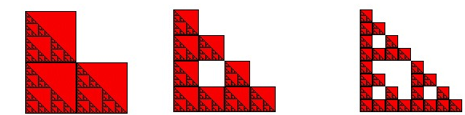
\includegraphics[width=1\textwidth]{Minskowski.PNG}
 \hspace*{1.25em} $r_1 = \frac{1}{2}$ $N(r_1)=3$
\hspace*{5em} $r_2 = \frac{1}{4}$ $N(r_2)=9$
\hspace*{7.75em} $r_3 = \frac{1}{8}$ $N(r_3)=27$


 Figura 2.15: Càlcul de la dimensió del triangle de Sierpinski amb el mètode de Box-counting
 \end{center}
En l'exemple del triangle de Sierpinski, obtenim com a resultat per a qualsevol valor de $r$ de 1,58, això és a causa de que es tracta d'un fractal autosemblant.
\newline
Aquest sistema es pot utilitzar virtualment a partir d'un ordinador, sent d'aquesta manera un dels mètodes més útils per calcular les dimensions dels fractals. Encara que no és l'únic ús que té. Aquest sistema també s'utilitza sovint en l'àmbit mèdic per al diagnòstic de malalties com podrien ser tumors, malformacions, coàguls de sang, malalties cerebrals, identificació de retina o fractures òssies.

També és útil en l'àmbit de la cartografia i l'arqueologia, ja que es tracta d'una manera versàtil de calcular les fronteres entre països, els canvis de desnivell o l'augment del nivell del mar.


\begin{center}
 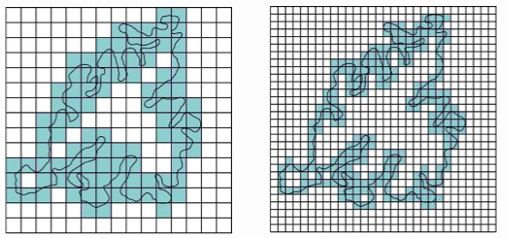
\includegraphics[width=1\textwidth]{Cartografia.PNG}
      Figura 2.16: Mètode del Box-counting aplicat a una superficie irregular
 \end{center}
\chapter{Fractals geomètrics}
\section{Fractals més clàssics} 
A continuació, parlarem d'alguns dels fractals més coneguts que hi ha. En aquest apartat, comentarem breument la història de com varen ser descoberts, els trets generals de cadascun dels fractals, i algunes de les propietats d'aquests (dimensió fractal, àrea...)
\subsection{Triangle de Sierpinski}
Començarem parlant del triangle de Sierpinski. Probablement, un dels fractals més coneguts i un dels més útils a l'hora d'explicar com és un fractal.
\newline
Aquest fractal va ser descobert l'any 1915 pel matemàtic polonès Waclaw Sierpiński. El que ell volia demostrar en el moment de la creació del fractal era que era possible la creació d'una corba que tenia perímetre infinit delimitant una àrea nul·la.
\newline
\begin{figure}
    \centering
   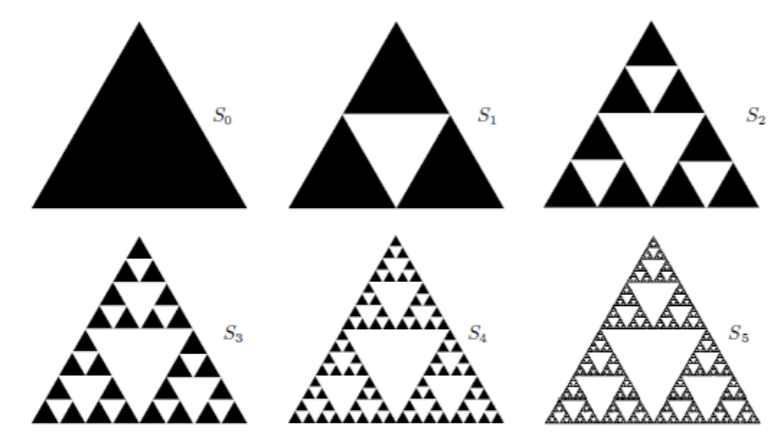
\includegraphics[width=0.59\textwidth]{triangle.PNG}
   \caption{Triangle de Sierpinski}
   \label{fig:my_label}
\end{figure}
Aquest és l'exemple més conegut del triangle de Sierpinski, el creat amb un triangle equilàter. Com es pot veure, aquesta figura ha estat formada extraient la part interior de cada triangle format dins d'aquesta. Així i tot, hi ha altres maneres de construir aquesta corba:

La primera i més senzilla és la que ja hem comentat, extraient la part interna de cada triangle que es forma. Amb aquest mètode, el que es fa és extreure la figura delimitada pels punts mitjans de cada un dels costats dels triangles formats a la iteració anterior. D'aquesta manera, per tant, la seva àrea es redueix 1/4 a la iteració anterior.

\begin{wrapfigure} {l} {0.4\textwidth}

    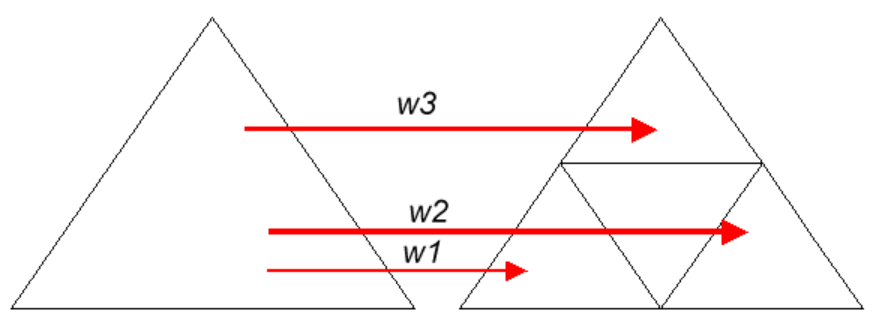
\includegraphics [width=0.4\textwidth] {sierpinski2.PNG}
    \caption{Sierpinski iterat}
\end{wrapfigure}
Un altre mètode per crear aquesta figura és a partir del reescalat i la translació de la figura. Primer es reescala la figura a 1/3 de la seva mida i s'aplica la translació per col·locar-la a tres punts diferents, ocupant 3/4 de l'àrea que ocupava la figura de la iteració anterior.

L'últim mètode, i el que podríem dir és el més curiós, es basa en el joc del caos. Aquest joc, del qual parlarem més endavant, utilitza una succeció de nombres aleatoris per tal de crear la imatge del triangle de Sierpinski.

A continuació parlarem de la longitud i l'àrea d'aquest fractal. Veient la figura que hem mostrat més amunt, podem deduir més o menys aquestes dues propietats. Encara i així, a continuació mostrarem dues taules per definir més detalladament la longitud i l'àrea d'aquest fractal a cada iteració.
\newline
\begin{itemize}
\item \textbf{Longitud}
\end{itemize}
Primer de tot, considerarem que el triangle inicial serà equilàter i que cadascun dels seus costats constarà d'una unitat de longitud.

\resizebox{14cm}{4cm}{
\begin{tabular}{|c |c |c |c |}
\hline
& Nombre de costats & Longitud de cada costat & Longitud total (en unitats
linears)\\
\hline

\newline
$S_0$ & $3\cdot1$ & $1$ & $3\cdot1=3$ \\[0,5cm]
\hline

$S_1$ & $3\cdot3$ & $\frac{1}{2}$ & $3\cdot3\cdot\frac{1}{2}=4,5$ \\[0,5cm]
\hline

$S_2$ & $3\cdot9$ & $\frac{1}{4}$ & $3\cdot9\cdot\frac{1}{4}=6,75$\\[0,5cm]
\hline

$S_3$ & $3\cdot27$ & $\frac{1}{8}$ & $3\cdot27\cdot\frac{1}{8}=10,125$\\[0,5cm]
\hline
$S_n$ & $3\cdot3^n$ & $\frac{1}{2^n}=(\frac{1}{2})^n$ & $3\cdot3^n\cdot(\frac{1}{2})^n=3\cdot(\frac{3}{2})^n$\\[0,5cm]
\hline
\end{tabular}
}
\newline
\newline
\newline
En la taula anterior se'ns mostren diferents dades sobre la longitud dels costats dels triangles depenent del número d'ells, sent $n$ el número de la iteració en la qual estem.
\newline
Per tal de calcular la longitud que tindrà la figura un cop es facin una infinitat d'iteracions, només s'ha de calcular la longitud total de la figura (última columna de la taula) fent que $n$ tendeixi cap a infinit. D'aquesta manera podem veure com la longitud que obtindrà el fractal serà infinita.
\newline
\newline
\newline
\newline
\newline
\newline
\newline
\newline
\newline
\newline
\newline
\newline
\newline
\begin{itemize}
\item \textbf{Àrea}
\end{itemize}
Considerem, un altre cop, que el triangle inicial sigui equilàter i que cadascun dels seus costats constarà d'una unitat de longitud, i que $n$ sigui el número de la iteració en la qual estem.
\newline
\newline
\newline
\hspace{-2em}
\resizebox{16cm}{4cm}{
\begin{tabular}{|c |c |c |c |c |c |} 
\hline
& \parbox{4em}{Nombre de\\ triangles}   &\parbox{6em}{Longitud de\\ la base de\\  cada triangle}   & \parbox{6em}{Longitud de\\ l'altura de\\  cada triangle} & Àrea de cada triangle & Àrea total\\
\hline
\newline
$S_0$ & $1$ & $1$ & $\frac {\sqrt {3}}{2}$ & $\frac{1}{2}$\cdot $1$\cdot {\frac {\sqrt {3}}{2}} & $1$ \cdot \frac{1}{2}\cdot $1$\cdot {\frac {\sqrt {3}}{2}}= $0,433...$\\[0,5cm]
\hline
$S_1$ & $3$ & $\frac{1}{2}$ &$\frac {\sqrt {3}}{4}$ & $\frac{1}{2}$\cdot \frac{1}{2}\cdot {\frac {\sqrt {3}}{4}} & $3$ \cdot \frac{1}{2}\cdot \frac{1}{2}\cdot {\frac {\sqrt {3}}{4}}= $0,324...$ \\[0,5cm]
\hline
$S_2$ & $9$ & $\frac{1}{4}$ & $\frac {\sqrt {3}}{8}$ & $\frac{1}{2}$\cdot \frac{1}{4}\cdot {\frac {\sqrt {3}}{8}} & $9$ \cdot \frac{1}{2}\cdot \frac{1}{4}\cdot {\frac {\sqrt {3}}{8}}= $0,243...$\\[0,5cm]
\hline
$S_3$ & $27$ & $\frac{1}{8}$ & $\frac {\sqrt {3}}{16}$ & $\frac{1}{2}$\cdot \frac{1}{8}\cdot {\frac {\sqrt {3}}{16}} & $27$ \cdot \frac{1}{2}\cdot \frac{1}{8}\cdot {\frac {\sqrt {3}}{16}}= $0,182...$\\[0,5cm]
\hline
$S_n$ & $3^n$ & $\frac{1}{2^n}=(\frac{1}{2})^n$ & $\frac {\sqrt {3}}{2^{n+1}}$ & $\frac{1}{2}$ \cdot \frac {1}{2^{n}} \cdot \frac {\sqrt {3}}{2^{n+1}}=\frac {\sqrt {3}}{2^{2n+2}} & $3^{n}$ \cdot \frac {\sqrt {3}}{2^{2n+2}}=\frac {\sqrt {3}}{4} \cdot (\frac{3}{4})^n \\[0,5cm]
\hline
\end{tabular}
}
\newline

A diferència del vist amb la longitud, l'àrea d'aquest fractal disminueix a cada iteració. A l'última columna de la taula veiem com a cada iteració es disminueix l'àrea, encara que cada cop menys en respecte a l'anterior. Així i tot, quan es facin infinites iteracions, l'àrea tendirà cap al 0 fins al punt d'arribar a ser nul·la.

Curiosament, aquest fractal no és l'únic "descobert" per Sierpinski, ja que hi ha variables del mateix com el tetraedre de Sierpinski que també són coneguts, encara que no els descriurem al ser massa similars.
\newpage
\subsection{Conjunt de Cantor}
Aquest curiós i simple fractal rep el seu nom del matemàtic i filòsof alemany Georg Cantor el qual, el 1883, el va utilitzar per a una de les seves investigacions més importants relacionada amb el "continu".
\newline
El conjunt de Cantor és considerat, per molts, el fractal més típic i conegut que hi ha, ja que és el més antic. El que també molts desconeixen, és que Georg Cantor no va ser el primer a treballar amb aquest fractal, ja que al 1875, el dublinès Henry John Stephen Smith, ja l'havia descobert però al morir abans de donar-lo a conèixer, Cantor va rebre tot el reconeixement.
\begin{figure}[H]
    \centering
   \includegraphics[width=0.75\textwidth]{cantor.PNG}
   \caption{Conjunt de Cantor}
\end{figure}
Aquest fractal permet dos definicions igualment vàlides per a la seva construcció:
\begin{itemize}
\item La definició numèrica ens diu que es tracta del conjunt de tots els punts de l'interval real [0,1] que permeten una expressió en base 3 que no utilitzi el dígit 1.
\end{itemize}
\begin{itemize}
\item Al mateix temps, la definició geomètrica ens indica que aquest fractal és de caràcter recursiu i que elimina, a cada iteració, el segment corresponent al terç central de cada interval.
\end{itemize}

Al ser un fractal bastant simple i fàcil d'entendre, ens dedicarem a detallar les primeres iteracions de la seva creació.
\newline
Primer de tot, tenim un segment [0,1] a la recta real, al qual li haurem d'extreure el segment equivalent al seu terç central, quedant dos segments de $\frac{1}{3}$ de la longitud del segment inicial. Els intervals resultants seran:
\newline
\newline
 \hspace*{13em}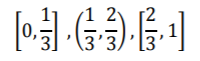
\includegraphics[width=0.3\textwidth]{cantor1.PNG}
 \newline
 Sent l'interval entre parèntesis el que hem d'extreure del segment original, quedant la primera iteració així:
 \newline
 \hspace*{13em}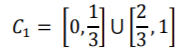
\includegraphics[width=0.3\textwidth]{cantor2.PNG}

Per a continuar amb el següent pas, haurem de repetir el mateix procès, però aplicant el que hem fet en la primera iteració a cadascun dels segments que ara hi ha. Els intervals que ara trobarem seran:
\newline
\hspace*{11em}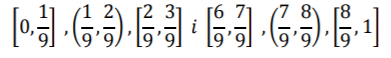
\includegraphics[width=0.5\textwidth]{cantor3.PNG}

A continuació, igual que hem fet abans, hem d'extreure tots els intervals entre parèntesis, ja que són els terços centrals corresponents per a cada segment.
\newline
\hspace*{11em}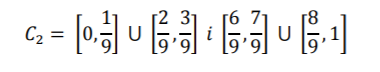
\includegraphics[width=0.5\textwidth]{cantor4.PNG}
\newline
Per acabar de crear el fractal sencer, hauríem de repetir aquest procés una infinitat de vegades, esborrant cada cop més segments però més petits, fins a arribar al punt on no podríem ni veure'ls al ser tan petits.
\newline
Un fet curiós d'aquest fractal és que, si fem els càlculs, veiem com arriba un punt on la longitud d'aquest és nul·la. El que és més curiós encara és que quan has fet una infinitat d'iteracions (sense que la longitud sigui zero), cadascun dels punts que trobem en el segment inicial tenen un punt corresponent (amb el que "s'emparellen") a la iteració en la qual estem. Això demostra com encara i ser un més petit que l'altre, la seva quantitat de punts en el segment són els mateixos, ja que ambdós són infinits.

Tal com hem fet abans, parlarem de la longitud del fractal, ja que no té àrea.
\newline
\newline
\newline
\newline
\newline
\newline

\begin{itemize}
\item \textbf{Longitud}
\end{itemize}
En aquest cas, el càlcul de la longitud és bastant més fàcil que el del triangle de Sierpinski, ja que es tracta simplement d'extreure troços del segment principal. També sabem que a cada iteració s'extreu una porció menor a la extreta en la iteració anterior.
\newline
\newline
\begin{tabular}{|c |c |c |c |}
\hline
& Nombre de segments & Longitud de cada segment & Longitud total \\
\hline

\newline
$C_0$ & $1$ & $1$ & $1$ \\[0,5cm]
\hline

$C_1$ & $2$ & $\frac{1}{3}$ & $2\cdot\frac{1}{3}=0,666...$ \\[0,5cm]
\hline

$C_2$ & $4$ & $\frac{1}{9}$ & $4\cdot\frac{1}{9}=0,444...$\\[0,5cm]
\hline

$C_3$ & $8$ & $\frac{1}{27}$ & $8\cdot\frac{1}{27}=0,296...$\\[0,5cm]
\hline
$C_n$ & $2^n$ & $\frac{1}{3^n}=(\frac{1}{3})^n$ & $2^n\cdot(\frac{1}{3})^n=(\frac{2}{3})^n$\\[0,5cm]
\hline
\end{tabular}
\newpage
\subsection{Corba de Koch}
El matemàtic suec, Helge von Koch, va introduir la corba que porta el seu nom al 1904 i com un exemple d'una corba contínua, infinita, i que no tenia tangent a cap dels seus punts.
\begin{figure}[H]
\hspace{4,85cm}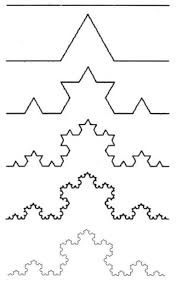
\includegraphics{koch.jpg}
\caption{Corba de Koch}
\end{figure}
Definirem el primer segment que veiem com a un format per l'interval [0,1]. La regla d'iteració que seguirà la creació d'aquest fractal seia: "Substituir la tercera part central de cada segment per dos segments de mida idèntica rotats amb un angle de 60˚ en sentits contraris, formant una dent."
\newline
Al aplicar la primera iteració, el segment que havíem vist abans s'ha "transformat" en un segment idèntic on s'ha substituït el terç central per un triangle equilàter sense base. Amb això obtindrem la primera corba, formada per quatre segments de $\frac{1}{3}$ de longitud cadascun.

Si repetim aquest procés infinites vegades, acabarem eliminant tots els terços centrals de cada segment creat amb anterioritat. Al substituir cadascun d'aquests fragments per dos segments a cada iteració, acabem tenint una corba de longitud infinita. Encara i així, un cop hem fet una infinitat d'iteracions, trobem imperceptibles els fragments que s'afegeixen, tot i que incrementen la longitud de la figura.

\begin{itemize}
\item \textbf{Longitud}
\end{itemize}
Ja que aquest segment està delimitat per l'interval [0,1], considerarem que aquest té una unitat de longitud amb la que treballarem per fer la taula següent:
\newline
\begin{tabular}{|c |c |c |c |}
\hline
& Nombre de segments & Longitud de cada segment & Longitud total \\
\hline

\newline
$C_0$ & $1$ & $1$ & $1$ \\[0,5cm]
\hline

$C_1$ & $4$ & $\frac{1}{3}$ & $4\cdot\frac{1}{3}=0,666...$ \\[0,5cm]
\hline

$C_2$ & $16$ & $\frac{1}{9}$ & $16\cdot\frac{1}{9}=0,444...$\\[0,5cm]
\hline

$C_3$ & $64$ & $\frac{1}{27}$ & $64\cdot\frac{1}{27}=0,296...$\\[0,5cm]
\hline
$C_n$ & $4^n$ & $\frac{1}{3^n}=(\frac{1}{3})^n$ & $4^n\cdot(\frac{1}{3})^n=(\frac{4}{3})^n$\\[0,5cm]
\hline
\end{tabular}
\newline
Com podem observar, la longitud total d'aquest fractal augmenta a cada iteració. Per tant, un cop fèssim infinites iteracions, trobariem que la seva longitud seria infinita.
\subsection{Floc de Koch}
Aquest fractal és una variació o extenció de la, anteriorment mencionada, corba de Koch, amb la qual comparteixen moltes propietats. Aquest fractal va ser creat pel mateix Koch uns anys després de crear la corba, al 1906. Aquest és, probablement, el fractal que a la gent més li sorprèn conèixer, ja que tothom l'identifica amb un floc de neu.
 \begin{figure} [H]
 \centering
  \subfloat{
    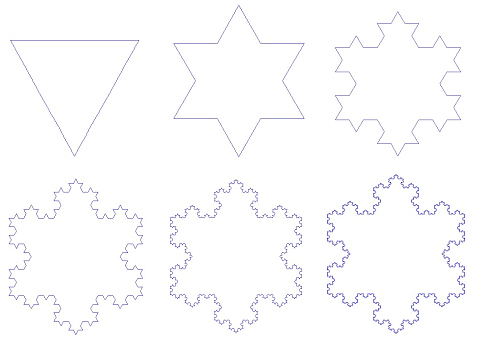
\includegraphics[width=0.57\textwidth]{floc.jpg}}
    \caption{Floc de Koch}
    \end{figure}
Com hem dit abans, les propietats d'aquest fractal són molt similars al anteriorment descrit. És per això que segueix la mateixa iteració que l'anterior, amb la única diferència que la figura inicial és un triangle equilater. 
\newline
Com a la corba de Koch, es substitueix cada segment per quatre de longitud menor. Continuant amb aquesta iteració una infinitat de vegades, obtenim el fractal.
\begin{itemize}
\item \textbf{Longitud}
\end{itemize}
Sabent que la longitud de la corba de Koch és $(\frac{4}{3})^n$, i que la longitud del cop de Koch és el triple que l'anterior, podem deduïr que la longitud del cop de Koch serà de $3\cdot(\frac{4}{3})^n$. 
\newline
Doncs, sabent que la longitud de la corba és infinita, la del cop també serà infinita.
\newline
\resizebox{16cm}{4cm}{
\begin{tabular}{|c |c |c |c |c |c |} 
\hline
& \parbox{4em}{Nombre de
\\triangles nous }   &\parbox{6em}{Longitud de\\ la base dels\\  nous triangles}   & \parbox{6em}{Longitud de\\ l'altura dels\\ nous triangles} & Àrea de cada triangle & Àrea total\\
\hline
\newline
$K_0$ & $0$ & $0$ & $0$ &$0$&  ${\frac {\sqrt {3}}{4}}= 0,433... $\\[0,5cm]
\hline
$K_1$ & $3$ & $\frac{1}{3}$ &$\frac {\sqrt {3}}{6}$ & $\frac{1}{2}$\cdot \frac{1}{3}\cdot {\frac {\sqrt {3}}{6}} & $A_K_0$+$3$ \cdot \frac{1}{2}\cdot \frac{1}{3}\cdot {\frac {\sqrt {3}}{6}}= $0,577...$ \\[0,5cm]
\hline
$K_2$ & $12$ & $\frac{1}{9}$ & $\frac {\sqrt {3}}{18}$ & $\frac{1}{2}$\cdot \frac{1}{9}\cdot {\frac {\sqrt {3}}{18}} & $A_K_0$+$A_K_1$+$12$ \cdot \frac{1}{2}\cdot \frac{1}{9}\cdot {\frac {\sqrt {3}}{18}}= $0,243...$\\[0,5cm]
\hline
$K_3$ & $48$ & $\frac{1}{27}$ & $\frac {\sqrt {3}}{54}$ & $\frac{1}{2}$\cdot \frac{1}{27}\cdot {\frac {\sqrt {3}}{54}} & $A_K_0$+$A_K_1$+$A_K_2$+$48$ \cdot \frac{1}{2}\cdot \frac{1}{8}\cdot {\frac {\sqrt {3}}{16}}= $0,182...$\\[0,5cm]
\hline
$K_n$ & $3^{n-1}$\cdot $3$ & $\frac{1}{3^n}=(\frac{1}{3})^n$ & $\frac {\sqrt {3}}{2\cdot3^n}$ & $\frac{1}{2}$ \cdot \frac {1}{3^{n}} \cdot \frac {\sqrt {3}}{2\cdot 3^n}=\frac {\sqrt {3}}{4\cdot3^{2n}} & $A_K_0$+···+4^{n-1}\cdot$3$\cdot\frac {\sqrt {3}}{4\cdot3^{2n}} \\[0,5cm]
\hline
\end{tabular}
}
\newline
\newline
\newline
Doncs, l'àrea total del floc de Koch quan les iteracions tendeixen a infinit seria:
\newline
\begin{figure}[H]
\hspace{4,3cm}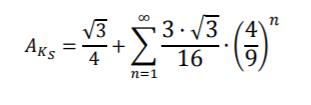
\includegraphics{areakoch.PNG}
\end{figure}
Amb això podem veure com una longitud infinita conté una àrea finita.
\newpage
\section{Construccions geomètriques iterades}
\justifying
Les construccions geomètriques iterades són repeticions d'uns certs processos, sempre idèntics, sobre un objecte geomètric.
És a dir, definim un sistema iterat com una funció que podem anomenar com $f(x_n)$ on $n \geq 0$, $x_1=f(x_0)$, al igual que $x_2=f(x_1)$ i així fins a $n=\infty$.
\newline
Mitjançant aquests processos podem ser capaços de construir qualsevol classe de fractal i fins i tot crear-ne de nous.
\newline
Aquestes iteracions estan formades per afinitats que són manipulades per un conjunt de normes: reescalat, translació i rotació. Repetint la iteració infinites vegades podem generar qualsevol fractal.
\newline
\begin{wrapfigure} {l} {0.3\textwidth}
    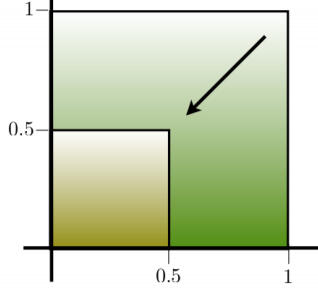
\includegraphics[width=0.24\textwidth]{Captura.PNG}
    \caption{Reescalat}
    \end{wrapfigure}
    \newline
    \newline
 El reescalat es basa en multiplicar dos valors; que anomenarem $\textbf{r}$ i $ \textbf{s}, sent\{r, s\} \in \mathbb{R}.$
    
\hspace{12em} $$
\begin{pmatrix}
X \\
Y \\
\end{pmatrix}
\mapsto
\begin{pmatrix}
Xr\\
Ys\\
\end{pmatrix} 
$$
\newline
\newline



\begin{wrapfigure} {r} {0.3\textwidth}
%\centering 
    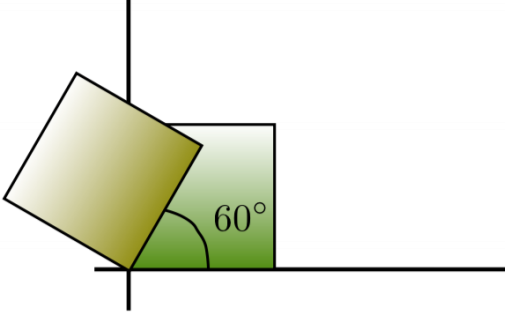
\includegraphics [width=0.3\textwidth] {rota.PNG}
    \caption{Rotació}
\end{wrapfigure}

La rotació funciona multiplicant la posició de l'objecte per la matriu
$\begin{pmatrix}
\cos{\theta} & -\sin{\varphi}\\
\sin{\theta} & \cos{\varphi}\\
\end{pmatrix} $
sent $\{\theta, \varphi\} \in \mathbb{R},$ 
 els valors angulars que vols que sigui rotat l'objecte.
\newline


$$\begin{pmatrix}
X \\
Y \\
\end{pmatrix}
\mapsto
\begin{pmatrix}
\cos{\theta} & -\sin{\varphi}\\
\sin{\theta} & \cos{\varphi}\\
\end{pmatrix} 
\begin{pmatrix}
X \\
Y \\
\end{pmatrix}
$$
\newline
\newline

\begin{wrapfigure}{l} {0.3\textwidth}
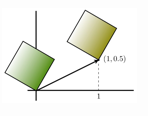
\includegraphics[width=0.3\textwidth]{traslacion.jpg}
\caption{Translació}
\end{wrapfigure}
 La translació consisteix en sumar a la posició de l'objecte un
valor per tal de desplaçar-lo. Ens referirem a aquest valor amb les lletres \textbf{e} i \textbf{h}, sent $\{e, h\} \in \mathbb{R},$ 
\newline
\newline
$$
\begin{pmatrix}
X \\
Y \\
\end{pmatrix}
\mapsto
\begin{pmatrix}
X\\
Y\\
\end{pmatrix} 
+
\begin{pmatrix}
e\\
h\\
\end{pmatrix} 
$$
\newline

\hspace{-10em} \begin{itemize}
    \item \textbf{Exemplificació mitjançant el triangle de Sierpinski}
\end{itemize} 
\begin{figure}[H]
    \centering
    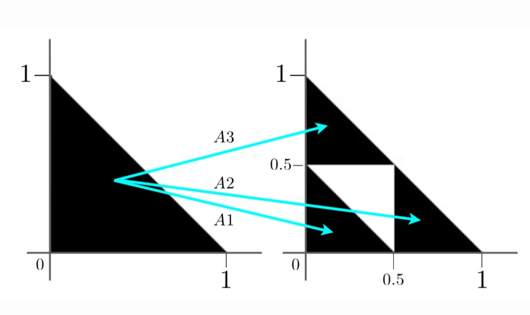
\includegraphics[width=0.7\textwidth,height=8\normalbaselineskip]{Iteracio1S.PNG}
    \caption{Iteracions}
\end{figure}


El triangle de Sierpinski es pot construir mitjançant dues de les tres possibles accions que podem aplicar, la translació i la reducció. En aquest cas necessitem aplicar-ho tres vegades, és a dir, per cada iteració estarem manipulant 3 afinitats.
\newline
Anomenarem $A_1$, $A_2$ i $A_3$ a la primera, segona i tercera afinitat, respectivament.
\newpage
\begin{wrapfigure}[43]{l}[0cm]{0.5\textwidth}
   \centering
    \vspace{-\normalbaselineskip}
    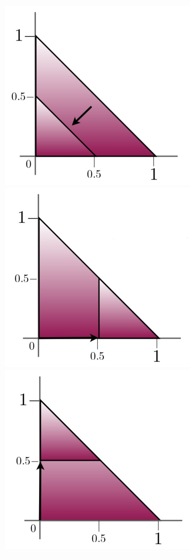
\includegraphics[width=0.25\textwidth,height=20\normalbaselineskip]{AfinitatsS.PNG}
    \caption{Afinitats}
\end{wrapfigure}  
\newline
\newline
\textbf{\underline{Primera afinitat $A_1$}:} 
\justifying
La primera afinitat únicament es basa en reescalar el triangle reduint els catets del triangle a la meitat.

$$reescalat: r=0.5$$
\textbf{\underline{Segona afinitat $A_2$}:} 
\newline
La segona afinitat reescala el triangle igual que a la primera afinitat però en aquest cas es trasllada 0,5 unitats de distància des del centre de coordenades en l'eix d'abscisses.
$$reescalat: r=0.5$$
$$traslaci\acute{o}:
\begin{pmatrix}
e\\
h\\
\end{pmatrix} 
=
\begin{pmatrix}
0.5\\
0\\
\end{pmatrix} $$
\textbf{\underline{Tercera afinitat $A_3$}:} 
\newline
La tercera afinitat és exactament igual a la segona exceptuant que la translació canvia. La tercera iteració es trasllada 0.5 unitats de distància des del centre de coordenades, però, en l'eix d'ordenades.
$$reescalat: r=0.5$$
$$traslaci\Acute{o}:
\begin{pmatrix}
e\\
h\\
\end{pmatrix} 
=
\begin{pmatrix}
0\\
0.5\\
\end{pmatrix} $$
\newline
\newline
\newline
\newline
\newline
\newline
\newline
\newline
\newline
\hspace{-3em}\begin{figure}
 Per tant, podem resumir la informació de la següent manera:
\end{figure}

\hspace{-8cm}   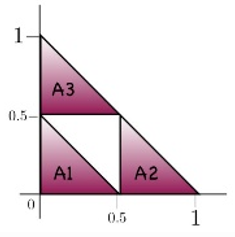
\includegraphics [width=0.2\textwidth] {A1A2A3.jpg}

\vspace{-8.5em} \hspace{-3em}
\begin{tabular}{|c |c |c |c |c |}
\hline
Afinitats & $r$ i $s$ & $\theta$ i $\varphi$& $e$ & $h$\\
\hline
$A_1$ & 0.5 & 0 & 0 & 0 \\
\hline
$A_2$ & 0.5 & 0 & 0.5 & 0 \\
\hline
$A_3$ & 0.5 & 0 & 0 & 0.5 \\
\hline
\end{tabular}
\newline
\newline
\newline 
Aquest conjunt de normes és al que ens referim com al sistema iterat del triangle de Sierpinski. Si repetim les iteracions infinites vegades, trobem que es genera el triangle de Sierpinski amb cada vegada més detall.
\newline
\begin{figure}[H]
 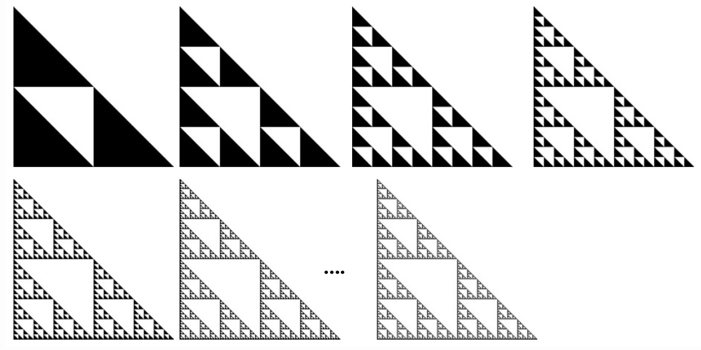
\includegraphics[width=1\textwidth]{IS.PNG}
 \caption{Iteració Triangle de Sierpinski}
 \end{figure}
\justifying

Concloem que, repetint les iteracions, es conserva la forma triangular. Per tant, podem canviar el generador per crear un fractal que, en l'infinit, es comporti igual que el Triangle de Sierpinski.
\newline
\begin{figure}[H]
 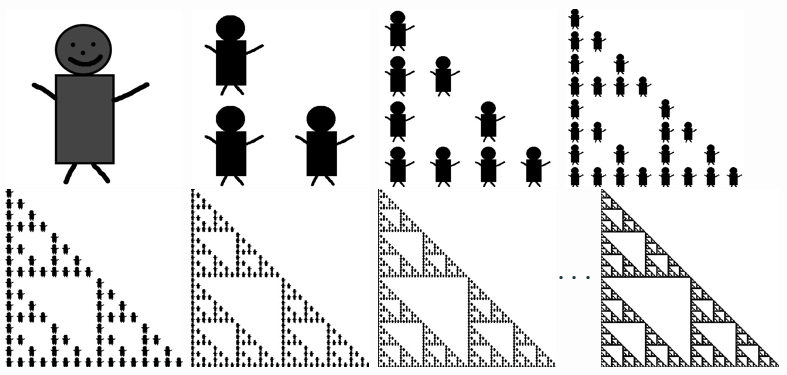
\includegraphics[width=1\textwidth]{IP.PNG}
 \caption{Exemple triangle de Sierpinski}
 \end{figure}
 \justifying
Sabem que un sistema iterat geomètric és un conjunt de contraccions en el pla $T_1$, $T_2$, ..., $T_n$, i $P_0$ qualsevol forma (o grup de punts).
\newline
Doncs la seqüència de generació de la forma del fractal seria:
\newline
$P_1=T_1(P_0)\cup ... \cup T_n(P_0)$
\newline
$P_2=T_1(P_1)\cup ... \cup T_n(P_1)$
\newline
\hspace*{5em} .
\newline
\hspace*{5em} .
\newline
\hspace*{5em} .
\newline
$P_{k+1}=T_1(P_k)\cup$ ... $\cup T_n(P_k)$
\newline
Si la seqüència convergeix en la figura $P$, doncs serà invariant a l'operació descrita.
$$P=T_1(P) \cup ... \cup T_n(P)$$
\newline
Sabent això, podem comprendre el \textcolor{magenta}{teorema de Collage}.
\newline
\newline
\newline
\newline
\newline
\begin{itemize}
    \item \textbf{Teorema de Collage}
\end{itemize} 
\justifying

Sigui $T_i$: $\mathbb{R}^2 \rightarrow \mathbb{R}^2$, on $i = 1$, ..., $N$ contraccions. Doncs $T$ : $K(\mathbb{R}^2) \rightarrow K(\mathbb{R}^2)$ serà la funció de collage, actuant sobre un conjunt compacte, un conjunt tancat i acotat, en el pla com
$$T(C) = T_1(C) \cup ... \cup T_n(C) = \bigcup_{k=1}^{N}P_k$$
on
$$T_i(C) = \{T_i(x,y); (x,y) \in C\}$$
sent 
$C$ un conjunt compacte $\in \mathbb{R}^2$
\newline
Doncs, existirà un únic conjunt $A$ que satisfagi
$$T(A) = A$$
El que provoca, per tant, és que per a qualsevol altre conjunt, diguem-ne $B$
$$\lim\limits_{k\to\infty} T^k(B) = A$$
amb les mesures de Hausdorff en k$(\mathbb{R}^2)$.
\newline
Un clar exemple del Teorema de Collage seria la Figura 3.12, vista en el punt anterior.
\section{Construccions geomètriques iterades aleatoriament mitjançant el joc del caos}
Les construccions geomètriques iterades aleatòriament són processos repetitius que es basen en l'atzar com a mitjà per a la construcció dels fractals. Aquests sistemes són molt sensibles als canvis i, com a resultat d'aquests, obtenim diferents tipus de fractals.
\begin{itemize}
    \item \textbf{El joc del caos}
\end{itemize} 
\justifying{Abans d'entrar en les matemàtiques darrere d'aquest joc, parlarem de com es juga i el resultat que té.
\newline
El joc del caos compleix un seguit de normes per al seu funcionament:
\begin{itemize}
\item [$-$] Ha de contenir un nombre major o igual a 2 punts assignats en l'espai que serveixin com a punts cardinals.
\end{itemize}
\begin{itemize}
\item [$-$] Els punts no han d'estar alineats.
\end{itemize}
\begin{itemize}
\item [$-$] Els punts han de ser estàtics en l'espai.
\end{itemize}
\begin{itemize}
\item [$-$] Ha d'existir un punt d'origen des d'on començar el joc, que sigui equivalent o no a un punt cardinal, contingut dins de la figura formada pels punts cardinals.
\end{itemize}
Per explicar el funcionament agafarem com a exemple la creació del triangle de sierpisnki mitjançant el joc del caos.
\newline
igui: $Q$,$P$,$S$ tres punts no alineats continguts en el pla $\mathbb{R}^2$ i un punt $z_0 \notin \{Q,P,S\}$ contingut en el pla $\mathbb{R}^2$. I sent la probabilitat d'escollir un dels tres punts la mateixa, és a dir, $\frac{1}{3}$.
\newline
Agafem al atzar un dels tres punts $Q,P,R$ per a definir el nou punt $z_1$.
\newline
Suposem que aleatoriament escollim el punt $Q$. Doncs, el nou punt $z_1$ serà, en aquest cas, el punt mitjà entre els punts $z_0$ i $Q$.
$$ z_1 = \frac{1}{2}\cdot\overrightarrow{Qz_0}+Q = \frac{1}{2}\cdot(z_0-Q)+Q = \frac{z_0+Q}{2}$$
I així succesivament sent $z_2 =  \frac{z_1+P}{2}$ (si aleatoriament escollim el punt $P$) fins a l'infinit.
\newline
Podem, doncs, expressar-ho com aplicar al atzar una de les tres aplicacións afins següents:
\begin{equation*}
\left.
\begin{aligned}
A_1(z_x) =  \frac{z_x+P}{2}\\
A_2(z_x) =  \frac{z_x+R}{2}\\
A_3(z_x) =  \frac{z_x+Q}{2}\\
\end{aligned}
\right\}
\end{equation*} 
\begin{figure}
També podem escriure la succcessió d'una manera més compacta
$$z_n = f^n(z_0)$$
sent $f$ el mecanisme aleatori, i per tant, ho podem interpretar com l'òrbita de $z_0$, la qual explicarem més endavant en l'apartat 4.2.1.
    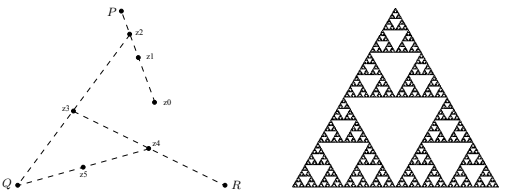
\includegraphics{PPQRQ.PNG}
    \caption{Esquerra: primers 6 punts en el joc del caos per lasequencia PPQRQ.... Dreta: Els seguents 80.000 punts.}
    \label{fig:my_label}
\end{figure}}
\begin{figure}
%\centering
    \hspace{7em} 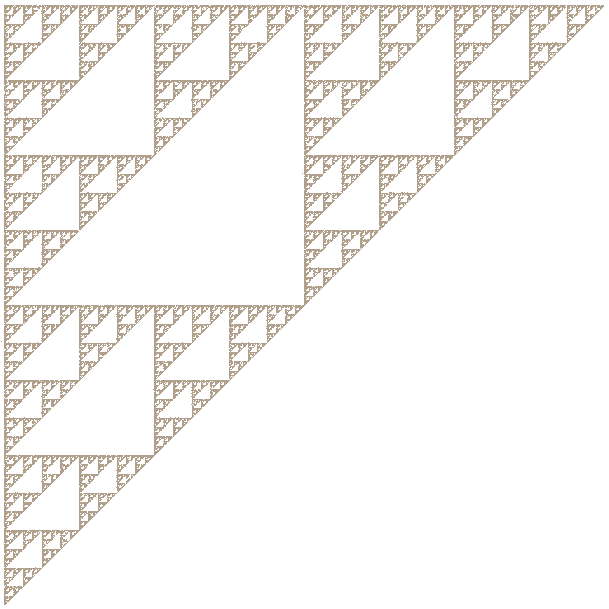
\includegraphics[width=0.7\textwidth]{TS1000000.PNG}
    \caption{Triangle de Sierpisnki amb 100.000 punts}
    \label{fig:my_label}
\end{figure}
\newpage
\justifying{
Modificant el valor de contracció, la quantitat i/o posició dels punts cardinals, afegint rotació o canviant la probabilitat, es poden generar fractals totalment diferents.
\newline
Aquest sistema per a la creació de fractals és molt útil i senzill de programar en sistemes informàtics, i és capaç de generar qualsevol classe de fractal que el programador pugui programar.
\newline
Com a exemple, nosaltres mateixos hem pogut programar diversos fractals, alguns coneguts, i d'altres de nous.}
\begin{itemize}
    \item \textbf{Programació d'un generador de fractals mitjançant el joc del caos amb C++}
    \newline 
\justifying{Per a dur a terme el programa vàrem decidir utilitzar com a llenguatge de programació el C++, utilitzant com a programa d'ajut SharpDevelop, ja que és un programa fàcil d'entendre, utilitzar, i ja que teníem nocions bàsiques del seu ús perquè vàrem tenir l'oportunitat d'aprendre a utilitzar-lo en l'assignatura d'informàtica en la nostra escola.
\newline
Com que bastanta part del programa és per a l'execució, així com la coordinació del mateix programa, farem menció únicament a les parts que tenen major importància sobre els càlculs i generació dels fractals. I obviarem les parts purament informàtiques.
\newline
\newline
El programa és una modificació d'un ja creat per a una tasca de l'assignatura d'informatica.
\newline
Per a accedir a tot el codi de programació, podeu anar a la pàgina 10 dels annexos.}
\begin{itemize}
    \item [$-$] \textbf{Programa de generació del Triangle de Sierpinski}
\end{itemize} 
\justifying{Per a la creació del fractal del Triangle de Sierpinski, necessitem anomenar dos variables claus. Una que consideri el nombre de punts que imprimirem per pantalla, ja que ens seria impossible fer-ho de forma infinita. I una que sigui el sistema aleatori que utilitzarem per a escollir a quin punt dirigir-nos.
\newline
Aquesta última variable és una Classe que ve per defecte anomenat Random que serveix per a la generació de nombres pseudoaleatoris. Anomenarem $rnd$ a la classe que generarà els nombres aleatoris.
\newline
Per altra banda, com que el nombre de punts que imprimirem per pantalla ha de ser un nombre natural d'un valor numèric relativament gran, utilitzarem una variable de tipus integuer ($\textcolor{naranja}{int}$) per a que guardi el valor. Aquesta variable l'anomenem numsprites.}
\newline
\newline
  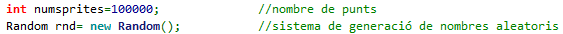
\includegraphics[width=0.9\textwidth]{numsprites.PNG}
  \newline
  \begin{list}{}
  \item \hspace{7em} Figura 3.15: Introducció de les variables
\end{list}

\begin{figure}
    \hspace{10em}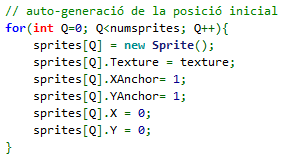
\includegraphics[width=0.5\textwidth]{posicioiniTS.PNG}
    \begin{list}{}
    \item \hspace{6em} {Figura 3.16: generació de la posició inicial dels punts} 
    \end{list}
\end{figure}
\justifying{Després de la declaració de les variables, en el que seria el set up, hi creem un bucle de tipus $\textcolor{blue}{for}$ per assignar a cada punt la seva textura i unes posicions a la pantalla per posteriorment reassignares.
\newline
Aquest pas serveix únicament per a que, posteriorment, assignar les coordenades correctes dels punts sigui més fàcil.}
\newpage
\begin{figure}
    \hspace{5em}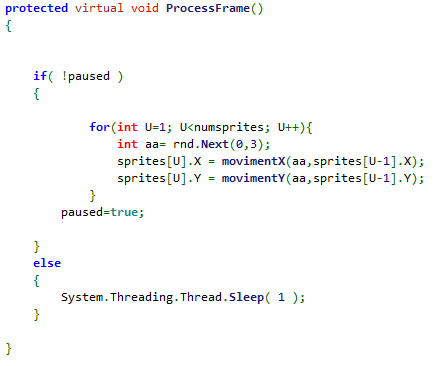
\includegraphics[width=0.8\textwidth]{processframeTS.PNG}
    \begin{list}{}
    \item \hspace{9em} {Figura 3.17: ProcessFrame del Programa} 
    \end{list}
\end{figure}
\justifying{El mètode del \textbf{\textcolor{blue}{ProcessFrame}}, encarregat de dur a terme els càlculs per a la posterior impressió dels mateixos per pantalla, està gestionat per una clau \textcolor{blue}{if} i una clau \textcolor{blue}{else}. 
\newline
En cas que el programa no estigui pausat, calcularà les coordenades dels punts. Per altra banda, si el programa està pausat, no calcularà res.
\newline
Per calcular les coordenades de tots els punts s'utilitza un bucle \textcolor{blue}{for}, ja anomenat anteriorment. En aquest, es calcula la posició de tots els punts utilitzant el sistema de nombres aleatoris i dos mètodes creats anomenats \textbf{\textcolor{blue}{movimentX}} i \textbf{\textcolor{blue}{movimentY}}.
\newline
Cada vegada que comença el bucle \textcolor{blue}{for}, el sistema de nombres aleatoris guarda dins de la variable de tipus integuer (\textcolor{naranja}{int} aa) un número entre el 0 i el 2, és a dir, tres números que corresponen a cada un dels punts cardinals necessaris per a la construcció del fractal.
\newline
Les coordenades dels punts es calculen basant-se en el nombre aleatori i en les coordenades del punt anterior. Per a facilitar els càlculs vàrem decidir descompondre les coordenades de cada punt en dos eixos l'eix X (eix d'abscisses) i l'eix Y (eix d'ordenades). Els mètodes \textbf{\textcolor{blue}{movimentX}} i \textbf{\textcolor{blue}{movimentY}} s'encarreguen de calcular el valor de la posició del seu eix corresponent.
\newline
Els dos mètodes són idèntics, l'única diferència és el valor de posició dels punts.
\newline
Eventualment, en finalitzar el bucle, es força al programa a aturar-se per a que no recalculi de forma infinita la posició de tots els punts i estigui canviant la posició dels mateixos sense parar.}
\newline

\begin{itemize}
    \item [$*$] \textbf{Métodes \textcolor{blue}{movimentX} i \textcolor{blue}{movimentY}}
\end{itemize}
     \hspace{2em}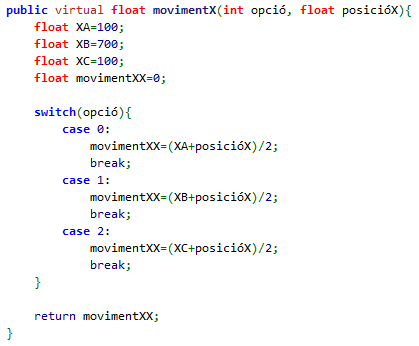
\includegraphics[width=0.7\textwidth]{movimentXTS.PNG}
     \newline
     \newline
     \newline
      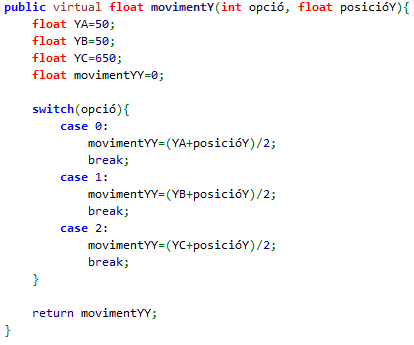
\includegraphics[width=0.7\textwidth]{movimentYTS.PNG}
     \newline
    \begin{list}{}
        \item \hspace{1em} {Figura 3.18: Mètodes de moviment X i Y} 
    \end{list}
    \vspace{3em}
    \justifying{
    Els mètodes calculen el valor de l'eix corresponent del nou punt calculant el punt mitjà entre el punt anterior del que estem calculant i un punt cardinal (en aquest cas anomenats $A,B$ i $C$).
\newline
Per a saber a quin punt cardinal es dirigirà, utilitzem la clau \textbf{\textcolor{blue}{switch}} amb la primera variable de tipus integuer (\textcolor{naranja}{int} opció) que fa referència a la variable que guarda el nombre aleatori.
\newline
Depenent el valor de la variable \textit{opció} es calcularà el punt mitjà entre el valor de l'eix del punt anterior; guardat en l'altre variable integuer (\textcolor{naranja}{int} posicióX, si és el mètode de \textcolor{blue}{movimentX} o posició Y si és el mètode de \textcolor{blue}{movimentY}).
\newline
El càlcul del punt mitjà és exactament igual que el ja abans explicar en l'explicació del joc del caos en la pàgina 33, l'únic que en comptes de calcular el punt mitjà entre els dos punts, calcula el valor mitjà de l'eix corresponent, de forma que quan es calculen els dos valors mitjans (un per cada eix), dóna el valor de la coordenada de la pantalla on primtar el punt.
    \newline
    \newline
    Ja al final del programa, en el mètode de dibuix anomenat \textbf{\textcolor{blue}{Render}}, existeix un últim bucle de tipus \textcolor{blue}{for} que serveix per a dibuixar tots els punts per pantalla sense necessitat de cap altre variable, ja que el punt mateix té les dades de tot al ser una variable de tipus \textbf{Class} que permet guardar dintre d'ella informació sobre la variable.}
    \newline
    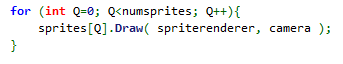
\includegraphics[width=0.7 \textwidth]{RenderTS.PNG}
    \begin{list}{}
        \item \hspace{5em}{Figura 3.19: Bucle de primtació dels punts per pantalla}
    \end{list}
    \newpage
    \begin{figure}
       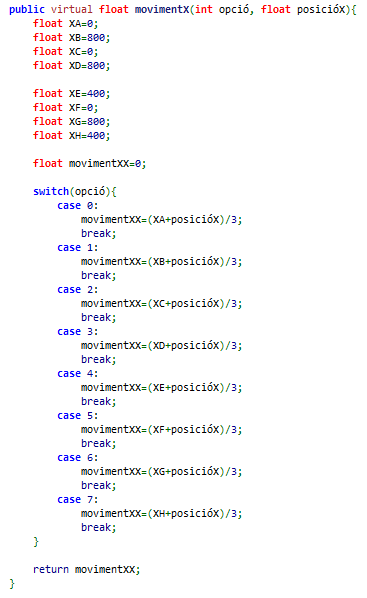
\includegraphics[width=0.53 \textwidth]{movimentXAlfombra.PNG}
        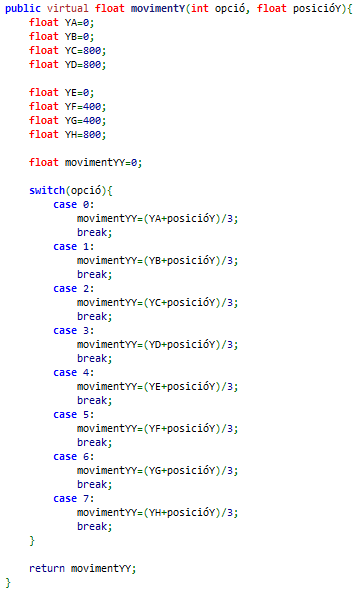
\includegraphics[width=0.53 \textwidth]{movimentYAlfombra.PNG}
         \begin{list}{}
        \item \hspace{1em} {Figura 3.20: Esquerra: mètode de movimentX per a la construcció de l'alfombra de Sierpisnki Dreta: mètode movimentY per a la construcció de l'alfombra de Sierpisnki} 
    \end{list}
       \hspace{12em} 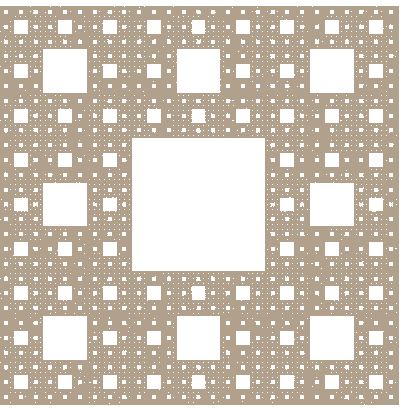
\includegraphics[width=0.4 \textwidth]{Alfombra.PNG}
        \begin{list}{}
        \item \hspace{10em} {Figura 3.21: Alfombra de Sierpinski} 
    \end{list}
    \end{figure}
    \newpage
    \begin{figure}
       \includegraphics[width=0.53 \textwidth]{MovimentXBoxI.PNG}
        \includegraphics[width=0.53 \textwidth]{MovimentYBoxI.PNG}
        \begin{list}{}
        \item \hspace{1em} {Figura 3.22: Esquerra: mètode movimentX per a la construcció del fractal de la caixa girat 90º Dreta: mètode movimentY per a la construcció del fractal de la caixa girat 90º} 
    \end{list}
       \hspace{12em} \includegraphics[width=0.4 \textwidth]{BoxI.PNG}
        \begin{list}{}
        \item \hspace{9.5em} {Figura 3.23: Fractal de la caixa girat} 
    \end{list}
    \end{figure}
    \newpage
    \begin{figure}
       \includegraphics[width=0.53 \textwidth]{MovimentXH.PNG}
        \includegraphics[width=0.53 \textwidth]{MovimentYH.PNG}
        \begin{list}{}
        \item \hspace{1em} {Figura 3.24: Esquerra: mètode movimentX per a la construcció del fractal del Hexàgon Dreta: mètode movimentY per a la construcció del fractal del Hexagon} 
    \end{list}
       \hspace{12em} \includegraphics[width=0.4 \textwidth]{Hexagon.PNG}
        \begin{list}{}
        \item \hspace{10em} {Figura 3.25: Fractal del Hexagon} 
    \end{list}
    \end{figure}
    \newpage
    \begin{figure}
        \includegraphics[width=0.53 \textwidth]{movimentXQuadratI.PNG}
        \includegraphics[width=0.53 \textwidth]{movimentYQuadratI.PNG}
        \begin{list}{}
        \item \hspace{1em} {Figura 3.26: Esquerra: mètode movimentX per a la construcció del fractal del Quadrat inclinat 90º Dreta: mètode movimentY per a la construcció del fractal del Quadrat inclinat 90º} 
    \end{list}
       \hspace{12em} \includegraphics[width=0.4 \textwidth]{QuadratI.PNG}
        \begin{list}{}
        \item \hspace{8.5em} {Figura 3.27: Fractal del Quadrat inclinat} 
    \end{list}
    \end{figure}
    \newpage
    \begin{figure}
       \includegraphics[width=0.53 \textwidth]{MovimentXCantor.PNG}
        \includegraphics[width=0.53 \textwidth]{MovimentYCantor.PNG}
        \begin{list}{}
        \item \hspace{1em} {Figura 3.28: Esquerra: mètode movimentX per a la construcció del Conjunt de Cantor Dreta: mètode movimentY per a la construcció del Conjunt de Cantor} 
    \end{list}
     \hspace{-2em} \includegraphics[width=3 \textwidth]{Cantor.PNG}
        \begin{list}{}
        \item \hspace{11em} {Figura 3.29: Conjunt de Cantor} 
    \end{list}
    \end{figure}
    \begin{itemize}
        \item [$\star$] \textbf{{\textcolor{red}{Observacions extretes a través de l'experimentació i recerca}}}
    \end{itemize}
    \justifying{
    Una vegada hem programat la generació del Triangle de Sierpinski, ens trobem que existeix una gran similitud entre el joc del caos, i el sistema geomètric iterat.
\newline
A més, visualitzem clarament una certa atracció en el joc del caos que provoca la creació del fractal.
\newline
Havent observat aquest comportament ens proposem construir altres fractals mitjançant el joc del caos, ja que sabent el perquè del seu funcionament, se'ns és bastant faci'l calcular la quantitat i posició de punts en el mapa per tal de crear els fractals.
\newline
Modificant el mètode movimentX i movimentY del programa del Triangle de Sierpinski, explicat en la pàgina anterior, hem sigut capaços de crear diversos fractals.
\newline
Ús deixem a les següents pàgines uns exemples d'altres fractals construïts per aquest sistema, explicant abans que les petites irregularitats i/o errors en la construcció dels fractals no és deguda a cap falla en el programa, poden ser degudes a errors decimals en els càlculs a l'hora de posicionar els punts cardinals i a la posició del punt inicial, ja que aquest no estava posicionat en un punt cardinal sinó en un punt qualsevol del pla, demostrant així, que des de qualsevol punt del pla es pot començar la generació del fractal sense haver-hi gairebé cap error, sent aquesta variable invariant en l'espai.}
\end{itemize}

\chapter{Fractals complexos i dinàmica complexa}
\section{Explicació dels Fractals Complexos}
Com ja vàrem introduir abans, a l'apartat de complexitat infinita, en la pàgina 12, faríem menció a dos diferents tipus de fractals. Els geomètrics, explicats durant tot el capítol 3, i els complexos.
\newline
Per a explicar aquests fractals, haurem d'introduir nous conceptes, així com la iteració de funcions, explicada en l'apartat 4.2.
\newline
A diferència dels fractals geomètrics, els fractals compostos no es poden explicar d'una manera senzilla a travès d'iteracions geomètriques repetitives. Els fractals complexos són productes d'iteracions de funcions complexes.
\newline
La creació dels fractals complexos és deguda a punts d'atracció i de repulsió que, aquests mateixos, generen al crear orbites, explicades en la pàgina 49.
\newline
Alguns dels fractals complexos més famosos són el conjunt de Julia o el conjunt de Mandelbrot, que explicarem i exposarem com a exemple en les següents pàgines.

\section{Iteració de funcions Complexes}  
Tal com ja hem explicat anteriorment, en l'apartat 3.2 a la pàgina 33, l'acte d'iterar és portar a terme un mateix procés repetides vegades. Anteriorment hem mencionat la iteració geomètrica; és a dir, la repetició de processos geomètrics. En aquest cas, la iteració d'una funció $F(x)$ és la composició d'aquesta amb ella mateixa: $F o F = F(F(x))$. D'aquesta manera, la funció en la primera iteració serà la variable, independentment de la segona iteració, tal que $F(x_n) = x_{n+1}$. Definirem la iteració n-èssima de la funció $F$ com $F^n$, per tant, $F^n = F o F^{n-1}$.
\newline
Sent $x_0$ el valor inicial (o llavor) d'on començarà la iteració, podem definir l'òrbita del valor $x_0$ com la successió de valors de $F(x)$:
$$x_0 \rightarrow x_1 = F(x) \rightarrow x_2 = F(x_1) = F^2(x_0) \rightarrow x_3 = F(x_2) = F^3(x_0) \rightarrow x_n = F^n(x_0)$$
\subsection{Iteració real quadràtica} 
Per tal de poder explicar la iteració de funcions complexes d'una manera més fàcil, ens dedicarem a explicar tota la base teòrica iterant funcions reals quadràtiques.
\newline
\newline
La iteració real quadràtica és la iteració de funcions expressades a partir d'un polinomi de grau 2 (quadràtic). $$F(x)= x^2 +k$$ sent $x$,$k \in \Re$, on $k$ és el paràmetre de la funció.
\newline
En funció del paràmetre obtenim diferents òrbites per a la funció les quals venen regides en funció dels punts fixes; punts que atrauen o repulsen la funció (encara que també poden ser neutres; és a dir, que no afectin a les òrbites de la funció).
\newline
Algebràicament podem trobar aquests punts fixes ressolent l'equació $f(x) = x$, que, en el cas d'equacions de segon grau, seria ressoldre l'equació: $f(x)=x \Rightarrow x^2+k = x \Rightarrow x^2-x+k = 0$.
\newline
Geomètricament, cal representar la funció $f(x)$ que iterarem i la bisectriu del primer i tercer quadrat (la funció identitat) $y=x$. Això és pel fet que aquesta, la funció identitat, és una funció afí on la imatge i l'antiimatge són sempre iguals. És per això que la intersecció entre la funció $f(x)$ i la bisectriu són els punts fixes de la funció, ja que compleixen la igualtat $f(x)=x$.
\newline
Cal, també, recalcar el tema de les progrecions geomètriques. Hem d'aclarir que quan el límit d'un conjunt o valor $k$ és multiplicat per si mateix $n$ vegades, i $n\rightarrow \infty$, el resultat variarà depenent del valor de $k$. 
\begin{itemize}
    \item [$-$]Si $k\in(-1,1)\Rightarrow\lim\limits_{x \rightarrow \infty}k^n=0$.
    \item [$-$]Si $k\in \mathbb{R}-(-1,1)\Rightarrow\lim\limits_{x \rightarrow \infty}k^n=\infty$.
    \item [$-$] Si $K$ és una funció, el resultat de $\lim\limits_{x \rightarrow \infty}k^n$ dependrà del valor de la seva llavor incial, i donarà lloc a diverses possibilitats que explicarem a continuació.
\end{itemize}
\begin{itemize}
        \item [$\bullet$] \textbf{Punts fixes atractors i repulsors}
        \newline
Essent $x$ un punt fix (que compleix la igualtat $f(x)=x$ i sent per tant un punt de tall entre $f(x)$ i la bisectriu $y=x$) el valor absolut de la primera derivada de la funció en el punt fix determinarà la seva naturalesa:
\begin{itemize}
    \item [$-$] Si $\arrowvert f(x) \arrowvert >1$ el punt fix $x$ és repulsor. Per exemple, la funció $f(x)=x^2-1$ té un punt fix a $x_0=\frac{1+\sqrt{5}}{2}$. El valor absolut de la primera derivada de la funció en el punt fix $x_0$ és major que 1, $f'(x_0)=1+\sqrt{5}>1 \Rightarrow x_0$ és un punt atractor, tal i com és pot observar a la Figura 4.1.
    \item [$-$] Si $\arrowvert f(x) \arrowvert <1$ el punt fix $x$ és atractor. Per exemple, la funció $f(x) = x^2-\frac{1}{2}$ té un punt fix a $x_0= \frac{1-\sqrt{3}}{2}$. El valor absolut de la primera derivada de la funció en el punt fix $x_0$ és menor que 1, $\arrowvert f'(x_0)\arrowvert= 1-\sqrt{3}<1 \Rightarrow x_0$ és un punt atractor, tal i com és pot observar a la Figura 4.2.
    \item [$-$] Si $\arrowvert f(x) \arrowvert =1$ el punt fix $x$ és neutre (encara que en alguns casos pot ser repulsor o atractor). Per exemple, la funció $f(x)=x^2-x$ té un punt fix a $x_0= 0$. El valor absolut de la primera derivada de la funció en el punt fix $x_0= 1$, $\arrowvert f'(x) \arrowvert=1 \Rightarrow x_0$ és un punt neutre ja que és mostra atractor per la banda esquerra i repulsor per la banda dreta; tal i com és pot observar a la Figura 4.3.
\end{itemize}
\end{itemize}
\begin{figure}
        \centering
        \includegraphics[width=0.4\textwidth]{f(x)repulsor.PNG}
        \caption{$f(x)=x^2-1$ tenint un punt fix repulsor}
        \label{fig:my_label}
\end{figure}
\begin{figure}
\centering
        \includegraphics[width=0.5\textwidth]{f(x)atractor.PNG}
        \caption{$f(x)=x^2-\frac{1}{2}$ tenint un punt fix atractor}
        \label{fig:my_label}
    \end{figure}
    \begin{figure}
\centering
        \includegraphics[width=0.6\textwidth]{f(x)neutre.PNG}
        \caption{$f(x)=x^2+x$ tenint un punt fix neutre}
        \label{fig:my_label}
    \end{figure}
\newpage
\begin{itemize}
    \item [$\bullet$] \textbf{Òrbites eventualment fixes}
    \newline
    Si partim d'una llavor $x_o$ es pot arribar a un iterat $x_n$ que sempre complirà la condició $f(x_n)=x_n$. Si la condició és compleix, l'òrbita de la llavor ($x_0$) s'anomenarà òrbita eventualment fixa. Com a exemple d'aquesta òrbita és l'òrbita de la funció $f(x)= x^2+k$ on $x_0=0$ i el paràmetre $k=-2$. Doncs, l'òrbita de $f(x=x_0)$ seria:
\end{itemize}
$$f(x_0)=-2 \rightarrow f(x_1)= f(x_0)^2-2= 2 \rightarrow f(x_2)=f(x_1)^2-2=2 \rightarrow f(x_3)= f(x_2)^2-2=2$$
\begin{itemize}
    \item [$\star$] \textcolor{red}{Observació}
    \newline
   Cal remarcar la semblança d'aquest tipus d'òrbites amb el teorema de Collage, ja que en el ja esmentat abans, a l'apartat 3.2 pàgina 38. En el susdit teorema per a qualsevol forma (en el que seria en aquest cas valor de $x_0$ que agafem que compleixi l'òrbita eventualment fixa) al cap d'infinites iteracions adquireix una mateixa forma concreta (el que seria el valor $x_n$).
\end{itemize}
\begin{itemize}
    \item [$\bullet$] \textbf{Òrbites $n$-periodiques}
    \newline
    Es tracta d'un conjunt de valors que procedeixen de les repeticions d'un cert nombre d'iteracions. Aquests períodes (o també anomenats cicles) indiquen el nombre mínim de punts que existeixen en l'òrbita tal que torna a arribar al punt inicial $x_n=x_0$. Aquest fenomen és anomenat com "tancar el cicle". La condició per a que un cicle sigui $n$-periodic és que $f^n(x_0)=x_0 \Leftrightarrow f^m(x_0) \neq x_0, \forall m \in \{1,...,n-1\}$ de forma que el valor d'$n$ ens indica el nombre d'iteracions que té el cicle (anomenat període).
\end{itemize}
 \begin{itemize}
    \item [$\star$] \textcolor{red}{Observació}
    \newline
  Mitjançant aquesta definició podem concloure que la principal característica d'aquests tipus d'òrbites és que contenen un nombre finit de punts. Així com podem afirmar que els punts fixes poden ser considerats cicles de període 1, $f^1(x_0)=x_0$.
   \newline
   \newline
\end{itemize}

\begin{itemize}
    \item \textbf{Òrbites eventualment periòdiques}
    \newline
   Les òrbites eventualment periòdiques, tal com es pot deduir pel seu nom, són òrbites que comencen per una llavor $x_0$ tal que inicialment no arriba a desencadenar un cicle; però que al cap d'un nombre indefinit d'iteracions arriba a un valor $x_n$ en el qual, finalment, s'inicia un cile $n$-periòdic que es tanqui en $x_n=x_u$. Perquè existeixi aquest tipus d'òrbites, s'haurà de complir una condició semblant a la de les òrbites $n$-periòdiques: $f^n(x_u)= x_n \Leftrightarrow f^m(x_u) \neq x_u, \forall m \in \{1, ..., n-1\}$. L'òrbita de la llavor $x_0$ que compleixi aquesta condició serà anomenada òrbita eventualment $n$-periòdica.
    \newline 
   Un exemple d'aquest tipus d'òrbites és la iteració de la funció real quadràtica de variable real $f(x)=x^2-1$; és a dir, quan el paràmetre d'una funció real de grau 2 és $k=-1$, per a la llavor $x_0=1$. L'òrbita d'aquesta funció per la llavor $x_0$ seria:
    $$1 \longmapsto 0 \longmapsto -1 \longmapsto 0 \longmapsto -1$$
    Que és tractaria d'un cicle 2-periodic.
    \item [$\star$]\textcolor{red}{Observació}
    \newline
   Observem que les orbites eventualment periòdiques tenen un comportament semblant a la generació de fractals geomètrics, anteriorment explicada en l'apartat 3.3 pàgina 39, en com des de qualsevol punt de l'espai es pot generar un fractal sent la variable del punt d'origen d'aquest invariable en l'espai, ja que aquest mateix acaba arribant a una òrbita fixa que eventualment, al repetir-se infinitament, acabarà generant el fractal.
    \item \textbf{Òrbites caòtiques}
    \newline
   Les òrbites caòtiques són aquelles que partint d'una llavor $x_0$, en cada iteració, l'òrbita no tendeix mai cap a cap cicle periòdic: s'escapa a infinit o no es veu condicionada per cap altra tipus d'òrbita. Manifesten un comportament erràtic, caòtic.
    \newline
    Un exemple d'aquesta òrbita és l'òrbita per a $x_0=0$ per a la funció $f(x)=x^2+0.5$, representada a la Figura 4.4.
\end{itemize}
\begin{center}
   \hspace{3em} \includegraphics [width=0.6 \textwidth] {f(x)caotic.PNG}
    \newline
    Figura 4.4: Òrbita de la funció $f(x)=x^2+0.5$ per a la llavor $x_0=0$
\end{center}
\begin{itemize}
    \item \textbf{Òrbita crítica}
    \newline
    En la iteració de funcions, la llavor més important és $x_0=0$. Aquest punt és anomenat punt crític; i a la seva òrbita, òrbita crítica.
    \newline
    És tant important aquesta llavor perquè representa el mínim de l'equació parabòlica $f(x)= x^2+k$; és a dir, que la seva primera derivada, $f'(x)=2x$, és igual a 0 per a $x_0=0$. I és que en funció del valor de l'ordenada a l'origen, el paràmetre $k$, que determina la posició de la funció en l'eix vertical, l'òrbita crítica escapa o no a l'infinit.
    \newline 
    \newline 
    Com a exemple d'aquesta òrbita també es pot observar en l'òrbita de $x_0=0$ de la funció $f(x)=x^2+0.5$ en la Figura 4.4.
\end{itemize}
\subsection{Iteració complexa lineal}
\subsubsection{Introducció als nombres complexos}
En el pla real, no existeixen arrels parelles de nombres negatius, per tant equacions com $x^2+1=0 \Rightarrow x^2 = -1 \Rightarrow x=\pm\sqrt{-1}$ no tenen solució real.
\newline
Per a poder resoldre aquest tipus d'equacions es va definir un conjunt de nombres, els nombres complexos, que vénen definits per l'expressió $z=a+bi$ on $z$ és el nombre complex que ve en funció dels paràmetres $a,b \in \mathbb{R}$; sent $a$ la part real del nombre complex i $b$ la seva part imaginaria, i sent $i$ la unitat imaginària equivalent a $\sqrt{-1}$.
\newline
L'expressió abans exposada, $z=a+bi$, s'anomena forma binòmia del complex però no és l'única forma d'expressar-los; per a poder multiplicar dos nombres complexos utilitzem la seva forma trigonomètrica.
\begin{center}
    \includegraphics[width=0.7 \textwidth]{Trigonometria.PNG}
    \newline
    Figura 4.5: Relació trigonometrica dels nombres complexos
\end{center}

Siguin $z_1= a+bi= r\cos{\alpha}+ r\sin{\alpha}i$ i $z_2=c+di= s\cos{\beta}+s\sin{\beta}i$ dos nombres complexos expressats de forma trigonomètrica, el producte seria: $z_1 \cdot z_2 = (a+bi)(c+di) = (rs\cos{\alpha}\cos{\beta}-rs\sin{\alpha}\sin{\beta})+(rs\cos{\alpha}\cos{\beta}+rs\sin{\alpha}\sin{\beta})i$.
\newline
Si apliquem les relacions trigonomètriques per a la suma de dos angles podem concloure que: $$z_1\cdot z_2=rs[\cos({\alpha+\beta})+\sin({\alpha+\beta})i]$$
Posteriorment, podem transformar el resultat obtingut en la forma polar, de tal manera que podem observar que $$z_1\cdot z_2 = r_\alpha \cdot s_\beta = (r \cdot s)_{\alpha+\beta}$$
\begin{itemize}
    \item Geometria de la Iteració complexa
    \newline
    En la Iteració complexa lienal no ens podem ajudar de la iteració gràfica per a visualitzar l'òrbita d'un nombre complex. Hem de calcular els iterats de l'òrbita a partir de la iteració algèbrica per posteriorment dibuixar-los en el pla complex i unir-los per mitjà de fletxes amb el sentit del nou iterat.
    \newline
    \newline
   En la iteració d'una funció de tipus $f(z)=az$, sent, per exemple, $a=i$. Es tracta de la multiplicació del nombre $z$ per la unitat imaginaria $i$; que en forma polar és $1_{90º}$. Per tant, com hem multiplicat el nombre complex $z$ per la unitat imaginaria, el mòdul inicial del producte és igual al mòdul del nombre complex $z$; mentre que el seu angle va augmentant en $90º$ cada vegada, tal com es pot observar en la Figura 4.5.
   \begin{center}
   \includegraphics[width=0.8 \textwidth]{orbitaradi1.PNG}
    \newline
    Figura 4.6: Iteració de $f(z) =zi$, observem que es manté en la circumferencia de radi 1 i es duplica l'angle.
\end{center}
   Si l'angle culpable de la rotació es tracta d'un nombre racional $\alpha= \frac{w}{T}$, com a l'exemple posat anteriorment, podem afirmar que l'òrbita realitzarà un cicle $n$-periòdic tal que $w$ determinarà el valor de voltes necessàries abans de tancar el cicle i $T$ determinarà el període de l'òrbita. En l'exemple anterior es tracta d'un cicle 4-periòdic que es tanca en la primera volta, ja que $\alpha=90º=\frac{1}{4}\cdot 360º$.
\item [$\star$] \textcolor{red}{Observació:} Teorema de Jacobi
\newline
També podem saber si una funció $f(z)=z^2+k$ produeix un cicle $n$-periòdic per a un valor $k$ si el paràmetre $k=e^{2\pi i \theta}, \theta \in \mathbb{R}$, ja que $\forall z_0 \in \mathbb{C} \hspace{0.25em} \backslash \hspace{0.25em} \{0\}$ l'òrbita de $z_0$ serà densa en la circumferència formada          $\{|z_0| = |z| \}$.
    \newline
    Aixó ve explicat pel \textcolor{magenta}{Teorema de Jacobi}
    \newline
    \newline
    \newline
   Si prenem ara la regla d'iteració $f(z)=az=\left( \frac{1}{2} + \frac{1}{2}i \right)z$ on el mòdul de $a$ és $r=\frac{1}{\sqrt{2}}<1$ i el seu argument $\alpha=45º$. Iterant la llavor $z_0=1$ som capaços d'observar com es produeix la rotació de $45º$ peró com els iterats de l'òrbita cada vegada s'apropen més a l'origen de coordenades. Això és a causa del fet que és multiplicat cada vegada per un mòdul inferior a 1; és a dir, l'eix de coordenades actua com a punt atractor tal com s'observa a la Figura 4.6.
    \begin{center}
        \includegraphics[width=0.8 \textwidth]{orbitaatractora.PNG}
    \newline
    Figura 4.7: $f(z)= \left( \frac{1}{2}+ \frac{1}{2}i \right)z$ tendeix cap a un punt fix atractor a l'origen de coordenades
    \end{center}
    El cas contrari és pot aconseguir per a la regla d'iteració $f(z)=az=(1+i)z$, on el mòdul de $a=\sqrt{2}>1$ i on el seu argument $\alpha=45º$. Iterant també de la llavor $z_0=1$, s'observa que es produeix la mateixa rotació, $45º$,però que té l'efecte contrari en l'òrbita, ja que aquesta s'allunya de l'eix de coordenades al ser multiplicada repetidament per un nombre major que $1$, com es pot observar en la Figura 4.7.
    \begin{center}
        \includegraphics[width=0.7 \textwidth]{orbitarepulsiva.PNG}
    \newline
    Figura 4.8: $f(z)= (1+i)z$ tendeix cap a un punt fix repulsor a l'origen de coordenades
    \end{center}
   Ens adonem, per tant, que les òrbites que traçarà la funció depenen del valor de $z_0$ i de $a$; és a dir, que com el punt fix és $z_0=0$, sempre que la llavor de l'òrbita no sigui 0 i el mòdul del valor anomenat $a$ no sigui igual a 0 ($|a| \neq 0$) l'òrbita traçada dependrà estrictament del valor del mòdul de $a$ de tal manera que si aquest és $<1$ serà atractor i si és $>;;;1$ repulsor. En cas que $|a|=1$ l'òrbita traçada és una circumferència.
\end{itemize}
\subsection{Iteració complexa quadràtica}
Es tracta d'iterar una funció complexa de variable complexa de grau dos; és a dir, iterar una funció de tipus $f(z)=z^2$, sent $z\in  \mathbb{C}$
\subsubsection{Geometria de la iteració}
Tal com hem dit abans, una funció complexa de grau 2, $f(z)=z^2$, es pot expressar perfectament com $f(z)=z \cdot z$. D'aquesta manera podem observar com les propietats de la iteració complexa lineal també es poden aplicar en les quadràtiques.
\newline
Igual que en la iteració lienal, expressarem les llavors en la seva forma polar; $z=r_\alpha$, amb
$r$ el seu mòdul i $\alpha$ el seu angle que forma amb l'eix d'abscisses.
\newline
Tal com vàrem explicar abans en l'apartat 4.2.2 en la pàgina 60, la multiplicació de dos nombres complexos és: $z_1 \cdot z_2 = r_\alpha \cdot s_\beta = (r \cdot s)_{\alpha+\beta}$. Té tal manera que quan $z_1 = z_2 =z$, el producte queda expressat d'aquesta forma: $z^2 = z \cdot z = r^2_{2\alpha}$. Així en les successives iteracions obtindrem, la següent òrbita:
$$z_0 = r_\alpha \mapsto z_1 = r^2_{2\alpha} \mapsto z_2 = r^4_{4\alpha} \mapsto z_3 = r^8_{8\alpha}$$
Per tant, deduïm que l'expressió general d'aquesta iteració en la seva forma polar és : $z_n=r^{2n}_{2\alpha}$; i en la forma trigonomètrica: $z_n=r^{2n}(\cos({2^n\alpha}) + \sin({2^n\alpha )i})$.
\newline
Però, caldrà diferenciar el comportament entre les llavors de mòdul igual, menor i major a 1.
\begin{itemize}
    \item Llavors de mòdul major a 1, $r>1$
    \newline
   Les llavors de mòdul $r>;;;;1$ corresponen als punts exteriors a la circumferència de radi 1. Com que el mòdul és major a 1, l'òrbita tendirà cap a infinit; és a dir, s'escaparà, ja que qualsevol nombre major a 1 al quadrat és sempre major al nombre original.
\item Llavors de mòdul menor a 1, $r<1$
\newline
Les llavors de mòdul $r<1$ corresponen a punts interiors a la circumferència de radi 1. Al contrari de les de mòdul $r>;;;;1$, que tendien a escapar, aquestes s'apropen cada vegada més al punt fixe al centre de coordenades.
    \begin{itemize}
        \item [$-$] Llavors iguals a 0
        \newline
        En el cas concret que el mòdul sigui igual a 0; és a dir, que la llavor $z_0=0$, l'òrbita d'aquest sempre serà el punt 0, ja que $f(0)=0^2=0$.
    \end{itemize} 
    \item Llavors de mòdul igual a 1, $r=1$
    \newline
    Les llavors de mòdul $r=1$ corresponen als punts pertanyents a la circumferència de radi 1 tal que el quadrat del mòdul d'aquestes llavors serà sempre $r^n=1$ i, per tant, tots els punts de l'òrbita d'aquesta llavor romandran en la circumferència unitària.
\newline
En aquest cas es dóna una rotació dels iterats al voltant de l'origen de coordenades que és determinat per l'angle $\alpha$ que es duplica en cada iteració.
\newline
    \newline
   Pel teorema fonamental de l'Àlgebra, sabem que tot polinomi de $n$ coeficients reals o complexos, té $n$ possibles solucions complexes o arrels. Per això, en la iteració complexa, sempre existeixen punts inicials l'òrbita dels quals és $m$-periòdica; $\forall m \in \mathbb{R}$. Això és pel fet que qualsevol polinomi mitjançant el qual cerquem l'òrbita $m$-periòdica de la funció tindrà solució; és a dir, punts en el pla complex en l'òrbita de període $m$.
    \newline
    En el cas de la iteració complexa quadràtica, $f(z)=z^2$, les òrbites periòdiques es donen únicament en la circumferència unitària, a excepció del punt fix $z=0$. Per això, les anomenem revolucions.
    \newline
    \newline
   Considerant el punt $z=1$ com 0 revolucions, el punt $z=i$ com $\frac{1}{4}$ revolucions, el punt $z=-1$ com $\frac{1}{2}$ revolucions i el punt $z=-i$ com $\frac{3}{4}$ revolucions; podem esbrinar el comportament d'aquestes llavors en la circumferència unitària. De tal manera que prenent la llavor $z_0=i$, o el que és equivalent, $\frac{1}{4}$ revolucions, observem una òrbita eventualment periòdica, explicades en la pàgina 49, al cap de dues iteracions, ja que en la iteració quadràtica l'angle sempre s'itera com $2\alpha$
    $$\frac{1}{4} \rightarrow \frac{1}{2} \rightarrow 1 = 0 \rightarrow 0 \rightarrow ...$$
    \item[$\star$] \textcolor{red}{Observació}
    Cal destacar que quan l'angle cau en el punt $z=1$ equivalent a 1 revolució, considerem que torna a 0 revolucions. 
    \newline
    Trobem també que una òrbita 2-periòdica si prenem la llavor $\frac{1}{3}$ revolucions: $\frac{1}{3} \rightarrow \frac{2}{3} \rightarrow \frac{1}{2} \rightarrow ...$.
    O una òrbita 3-periòdica si  iniciem l'òrbita amb la llavor $\frac{3}{7}$ revolucions: $\frac{3}{7} \rightarrow \frac{6}{7} \rightarrow \frac{5}{7} \rightarrow \frac{3}{7} \rightarrow \frac{6}{7} \rightarrow ... $.
    \newline
    Per tant, les òrbites de les llavors seran $m$-periòdiques o eventualment periòdiques $\Leftrightarrow$ el valor de la llavor es pot expressar com un nombre racional. En canvi, quan l'angle de les llavors de la circumferència unitària s'expressa mitjançant un nombre irracional, l'òrbita d'aquestes llavors no formarà cap cicle sinó que omplirà densament la circumferència unitària.
    \end{itemize}
\section{Analisis dels fractals complexos més coneguts}
Una vegada explicat el funcionament de la iteració complexa, som capaços d'explicar la formació de diversos tipus de fractals complexos, així com el conjunt de Julia o el conjunt de Mandelbrot.
\subsection{Conjunt de Julia}
El conjunt de Julia, anomenat en honor al matemàtic francès Gaston Julia, és una família de conjunts de nombres complexos de la funció $f(z)=z^2+k$ en funció del paràmetre $k$.
\begin{center}
    \includegraphics[width=1 \textwidth]{Julia.png}
    Figura 4.9: Representació del Conjunt de Julia
\end{center}
Com ja hem explicat anteriorment a l'apartat 4.2.1, les òrbites d'una funció complexa $f(z)$ es poden distingir segons com es comporten; és a dir, quina és la seva tendència: a formar cicles, escapar a l'infinit o a ser atret a un punt fix.
\newline
En funció d'aquestes tendències som capaços de distingir dos conjunts que, a la vegada, són complementaris.
\begin{itemize}
   \item \underline{Conjunt de Julia ple}
    

   Un conjunt de Julia ple ($K_f$ per a $f(z)=z^2$) és aquell que les òrbites de cada llavor $z$ convergeixen a un punt fix atractor situat a l'interior de la circumferència unitària o bé pertanyen o tendeixen a formar cicles $n$-periòdics.
    \newline
   Per tant, en aquest conjunt, les òrbites dels seus punts pertanyeran a l'interior de la circumferència unitària. Així, per a la funció $f(z)=z^2$, podem definir un conjunt$K_f$, i el conjunt de Julia ple corresponent, com:
    $$K_f:=\{z \in  \mathbb{C} \hspace{0.25em} \backslash \hspace{0.25em} |z| <1\}$$
    En general, per a tota funció de la forma $f(z)=z^2+k$, el conjunt de Julia ple s'expressa com:
    $$K_f := \{ z_0 \in \mathbb{C} \hspace{0.25em} \backslash \hspace{0.25em} f^n_k(z_0) \nrightarrow \infty \hspace{0.5em} \text{quan} \hspace{0.5em} n \rightarrow \infty \}$$
    En aquest cas, per a calcular el valor del mòdul de la llavor $z_0$ a partir del qual escaparà cap a infinit cal trobar el valor d'escapament $E(k)$ que definirem més endavant.
    \newline
    Si $K_f$ compleix la seva definició, complirà també un seguit de propietats que mostren el seu caràcter fractal:
\end{itemize}
   
    \begin{itemize}
        \item [$-$] $K_f$ és compacte, no numerable i sense cap punt aïllat
        \item [$-$] $K_f$ és igual rere $n$ iteracions $\Leftrightarrow k$ sigui constant ja que $K_f=K^n_f$ on $n \in \mathbb{N}$
         \item [$-$] $K_f$ és invariant per a $f(z)$ i $f^{-1}(z)$
   
    \item \underline{Conjunt de Julia}
    \newline
    Un conjunt de Julia, $J_f$, es defineix com la frontera entre aquells punts que tenen òrbites que escapen a infinit i aquells que no.
    \newline
    Per tant, considerant $J_f$ qualsevol conjunt de Julia de la funció $f(z)=z^2+k$, defimin aquest com:
   \end{itemize} 
   $$ J_f := \{ z_0 \in \mathbb{C} \hspace{0.25em} \backslash \hspace{0.25em} f^n_k \nrightarrow \infty \hspace{0.25em} \text{quan} \hspace{0.25em} n \rightarrow \infty \hspace{0.25em} \text{on} \hspace{0.25em} \exists \hspace{0.25em} z'_0 \hspace{0.25em} \text{adjecent a} \hspace{0.25em} z_0 \hspace{0.25em} / \hspace{0.25em} f^n_k(z'_0) \rightarrow \infty \hspace{0.25em} \text{quan} \hspace{0.25em} n \rightarrow \infty \}$$
\begin{itemize}
    \item [$ $] Per a expressar el comportament de les òrbites de les llavors en el Conjunt de Julia, és necessari introduir l'expressió de cada punt de la circumferència unitària en revolucions; ja esmentat anteriorment en l'apartat 4.2.3 a la pàgina 54.
    \newline
    Després d'iterar un nombre complex, si el valor de la revolució és major o igual al valor de la revolució abans d'iterar-ho, es reduirà el seu valor a una revolució equivalent entre 0 i 1.
    \newline
    D'aquesta manera, si iterem la llavor $z_0=i$ per a la funció $f(z)=z^2$, l'òrbita serà:
    $$\frac{1}{2} \rightarrow \frac{1}{4} \rightarrow 1 = 0 \rightarrow 0 \rightarrow ...$$
    \item [$\star$] \textcolor{red}{Observació}
    \newline
    Aquesta òrbita es trobarà al punt $z=1$; és a dir, a 0 revolucions. Per tant, tendirà a aquest punt fix.
\end{itemize}
\subsubsection{Valor d'escapament}
\begin{itemize}
    \item Calcul:
    \newline
    El valor d'escapament $E(k)$ per a la funció $f(z)=z^2+k$ indica per a quins valors de $k$ la iteració d'aquesta funció escaparà a l'infinit i, per tant, no formarà part de Conjunt de Julia.
    \newline
    Definim el valor d'escapament com $E(k):= max\{|k|,2\}$; de forma que si $|k|>2$ afirmem que $|f^n(z_0)|> E(k) \Rightarrow f^n_k(z)\rightarrow \infty$, l'òrbita escaparà a l'infinit.
    \newline
    Per tal de conèixer el valor d'escapament, $E(k)$, d'una funció $f(z)=^2+k$, hem de calcular el mòdul del paràmetre complex $k$, sent $k=a+bi$, $|k|= \sqrt{a^2+b^2}$.
    \newline
    Depenent del valor del mòdul d'escapament trobem diferents valors d'escapament; és a dir:
    \begin{itemize}
        \item [$-$] $|k| \leq 2 \Rightarrow 2$
        \item [$-$] $|k| > 2 \Rightarrow |k|$
    \end{itemize}
   Observem, doncs, que el Conjunt de Julia pot estar contingut per una circumferència de radi 2 o bé per la circumferència de radi $|k|$, $\Leftrightarrow|k|>2$.
    \newline
    Per tant, el valor d'escapament serà aquell valor del mòdul de $k$ superior a 2 o, per defecte, 2.
    \item \textbf{Demostració}
    \newline
    Demostrarem en aquest apartar perquè la funció $f(z)=z^2+k$, un punt escaparà a infinit quan aquest superi el valor d'escapament; és a dir, quan $|z_n|>E(k)$.
    \newline
   Partint de l'hipòtesis que $z_n$ és un dels punts de l'òrbita d'una llavor i que $|z_n|>E(k)$. 
    \newline 
   Expressem la desigualtat triangular en la forma $|A+B| \geq |A|-|B|$, recordem que en tot moment representem un nombre complex com un triangle des de l'origen de coordenades.
    \newline
    Per tant, podem extrapolar:
    $$|z_n^2+k| \geq |z_n^2| -|k| \Rightarrow |z_n+1| = |z_n^2+k| \geq |z_n^2| - |k|$$
    Si $|z_n|>E(k)$,
    $$|z_n|>|k|, \hspace{0.5em}\text{per tant}, \hspace{0.5em} -|z_n| < -|k|$$
    Doncs:
    $$|z_{n+1}| \geq |z_n|^2-|k| > |z_n|^2-|z_n|=|z_n|\cdot(|z_n|-1) \hspace{1em}(\ast)$$
    Sabent per definició que $|z_n|>2$, deduïm de l'expressió anterior que $|z_n|-1>1$. 
    \newline
    Si expressem $D \sim (|z_n|-1)$, que, necessariament, $D>1$; podem deduïr de $(\ast)$
    $$|z_{n+1}|>D\cdot |z_n|$$
    Si $|z_{n+1}|>|z_n|$ per un factor $D>1 \Rightarrow|z_{n+1}| \rightarrow \infty$.
    \newline
    També, podem demostrar que $|z_{n+2}|>D^2|z_n|$ pel mètode d'Inducció, explicat i demostrat més endavant.
    \newline
    En general, diem que:
    $$|z_{n+k}|=D^k|z_n|$$
    \item[$\star$] \textcolor{red}{Observació}
    \newline
    Observem que si $D>1, D^k$ creix de manera que $|z_{n+k}|\rightarrow\infty$. Per tant, l'òrbita de qualsevol llavor de mòdul que superi el valor d'escapament, escaparà a l'infinit.
    \newline
    D'igual manera, podem observar que si  $D<1, D^k$ decreix de manera que $|z_{n+k}| \rightarrow 0$
    
    \item \textbf{Demostració mitjançant el mètode d'Inducció}
    \newline
    Demostrarem que $|z_{n+2}|>D^2|z_n|$ pel mètode d'Inducció:
\newline
\newline
Sabem que: $|z_{n+1}|>D\cdot |z_n|$
\newline
Ho anem a demostrar per a $n+1$
\newline
 $|z_{n+1+1}|>D \cdot |z_{n+1}| \Longrightarrow |z_{n+2}| > D \cdot D \cdot |z_n| = D^2|z_n|$ 
 \newline
 Com que l'expressió és vàlida, podem concloure que hem demostrat que
 $$|z_{n+k}|>D^k|z_n|$$
 O en general
 $$|z_{n+k}|=D^k|z_n|$$
\end{itemize}
\subsection{Conjunt de Mandelbort}
Com hem pogut observar en els apartats anteriors, podem diferenciar els fractals que s'obtenen a partir de la iteració de la funció $f(z)=z^2+k$ en dos grups que depenen dels comportaments de les llavors del pla amb el paràmetre $k$: els fractals connexes (on l'òrbita crítica no escapa a l'infinit) i la pols fractal (aquells que l'òrbita si escapa a l'infinit).
\newline
El conjunt de Mandelbort és el conjunt de paràmetres $k$ en que l'òrbita crítica de la iteració $f(z)=z^2+k$ no escapa a l'infinit.
\newline
Per tant, podem definir el conjunt de Mandlbort com:
$$M := \{ k \in \mathbb{C} \hspace{0.25em} \backslash
\hspace{0.25em} K_k \hspace{0.5em} \text{és connex} \hspace{0.5em}\}$$
és a dir,
$$M := \{ k\in \mathbb{C} \hspace{0.25em} \backslash \hspace{0.25em} f^K_k(0)\nrightarrow \infty\}$$
 El Conjunt de Mandelbrot es troba dins de la circumferència de radi 2 que té com a centre l'origen de coordenades, tal com es pot observar a la figura 4.8.
 \begin{center}
     \includegraphics[width=0.5 \textwidth]{mandelbortCr2.png}
     \newline
     Figura 4.10: Conjunt de Mandelbort
 \end{center}
També, observem com el Conjunt de Mandelbrot té simetria respecte a l'eix d'abscisses però no té simetria des de l'eix d'ordenades.
\newline
El Conjunt de Mandelbrot, està format per un cardioide principal, anomenat així perquè el seu límit és similar a la corba matemàtica cardioide.
\newline
Enganxades a la cardioide principal, trobem les components hiperbòliques, regions circular, definides posteriorment, de les quals sorgeixen moltes altres components hiperbòliques i antenes que, es toquen entre elles en un punt d'unió.
 \newline
 \begin{itemize}
 \justifying
     \item \textbf{Components hiperbòliques}
     \newline
 Les components hiperbòliques estan caracteritzades perquè els punts del seu interior convergeixen al centre de la component, en comptes d'escapar a l'infinit.
\newline
El centre de la component hiperbòlica és el punt que té un període determinat tal que l'òrbita crítica del component en el punt retorna a 0; per tant, ha de ser periòdica o eventualment periòdica.
En aquest punt la iteració de la funció $Q_k(z)=z^2+k$ rere $k$ iteracions s'expressa com $Q^t_k(0)=0$.
 \newline
 El centre de cada component hiperbòlic es correspon al valor $k$ tal que l'òrbita periòdica tractora de la funció $Q_k(z)$ té multiplicador $\mu =0$ ja que un dels factors del producte  $\mu$ és $|Q'_k(z_i)|= 2z_i = 0$ ja que $z_i=0$, i essent $\mu$ com: 
 $$\mu = |Q'k(z_0)| \cdot |Q'_k(z_1)| \cdot ... \cdot |Q_k(z_{t-1})| = \prod_{j=0}^{t-1} |Q'_k(z_j)| $$
 \end{itemize}
\chapter{Conclusions i bibliografia}
\section{Conclusions}
Com s'ha vist al llarg del nostre treball, hem volgut aprofundir en els aspectes més geomètrics i clàssics del món dels fractals, junt amb les matemàtiques necessàries per fer-ho. En un principi anàvem a centrar, exclusivament, el nostre treball en aquest tipus de fractals però, a mesura que avançàvem amb la nostra recerca, ens hem anat adonant que seria necessària la introducció dels fractals complexos.
\newline
\newline
El procés de redacció ha estat l'adequat, ja que hem pogut aprendre a utilitzar l'aplicació de LaTeX, junt amb altres eines i coneixements que ens han ajudat al desenvolupament del treball. En un principi se'ns va fer difícil treballar amb aquest nou programa, però ens hem adaptat correctament i hem tirat endavant. Junt amb això, hem enfocat el nostre projecte de la manera que teníem previst, i podem dir que estem molt orgullosos de la feina feta.
\newline
\newline
Hem pogut parlar de la història dels fractals i de molts d'ells en detall, al mateix temps que treballàvem en la programació i creació d'aquests. De la mateixa manera que vam tenir problemes amb el funcionament de LaTeX, l'inici no va ser senzill per la programació dels fractals, ja que requeríem de coneixements que no sabíem i vam haver d'investigar i practicar molt abans d'aconseguir resultats. També hem pogut entendre la importància de les matemàtiques al nostre dia a dia i, gràcies a això, hem obtingut una visió diferent del que ens rodeja i de la geometria que coneixem.
\newline
\newline
Al llarg del nostre treball, hem entès que no sempre sortirà tot com creiem, per molt bé que es planifiqui. Hi ha coses que no depenen de nosaltres, i hem hagut d'aprendre a adaptar-nos sobre la marxa. També ha sigut necessària la comunicació amb la Universitat de Barcelona, i el contacte amb un estudiant d'allà, el David Balbuena, el qual ens ha assessorat i ajudat tant en l'àmbit del treball com en el nostre creixement personal, ja que requeríem d'una certa professionalitat.
\newline
\newline
Clarament, el treball ha estat una experiència gratificant tot i el temps i esforços dedicats. Ha estat la primera vegada que hem treballat durant un termini tan llarg de temps, i podem dir, convençuts, que ha sortit bé. Com ja hem dit abans, han sorgit alguns inconvenients, però hem aconseguit afrontar-los i superar-los tots ells. Cal recalcar el gran esforç que ens ha suposat, sobretot cap a inicis de segon de Batxillerat, el fet de compaginar l'avanç del treball amb les assignatures escolars, ja que el nostre ritme a l'estiu va ser molt elevat i vam veure un gran canvi al retornar a fer classes. Així i tot, tot ha sortit molt bé i estem molt conformes amb els resultats.

\section{Agraïments}
El nostre treball de recerca ha estat supervisat per Pedro Román, a qui ens agradaria expressar el nostre agraïment, per a fer possible la realització d'aquest treball. A més, agrair la seva paciència i dedicació que ha tingut per ajudar-nos a fer que tot surti exitosament. Gràcies pel teu suport.
\newline
També volem agrair a dos membres de la UB. A la nostra coordinadora Nuria Fagella, per donar-nos la possibilitat de fer aquest treball, i al nostre tutor David Balbuena el qual ens ha estat indispensable per a l'assoliment del treball.
\newline
Per acabar, també volem agrair als nostres familiars i amics, els quals ens han donat suport durant aquest llarg trajecte, sense deixar-nos mai caure i estant sempre allà.
\newline
I, com no podia ser de cap altra manera, donem les gràcies a les matemàtiques i als fractals per ser, un altre cop, una font de coneixement i d'inspiració per a les nostres vides.
\section{Bibliografia i Webgrafia}
[CDF] J. Choate, R.L. Devaney, A. Foster. Fractals (A tool kit of dynamics activities).
Key Curriculum Press 1999. ISBN 1-55953-355-2.
\newline
\newline
[FJ] N. Fagella i X. Jarque, Iteración Compleja y Fractales. Coed. Vicens Vives/ICE
(UAB), 2007. col·lección enseñar y saber en el Siglo XXI.
\newline
\newline
[D] R.L.Devaney, A first course in Chaotic Dynamical Systems. Addison-Wesley
1992.
\newline
\newline
[P] H.O.Peitgen, Dietmar Saupe, (editors), The Science of fractal images. Springer,
1988.
\newline
\newline
[B] M.F. Barnsley, Fractals everywhere. Academic Press, 1988.
\newline
\newline
[MF] http://www.maia.ub.es/holodyn/mathfrac Software Mathfrac creat per
Christian Mannes pel nostre grup. Amb aquest programa es poden explorar
els fractals resultants d’un IFS.
\newline
\newline
[W1] http://math.bu.edu/DYSYS Web amb informació sobre fractals (i altres
aspectes d'iteració) totalment adaptada a alumnes de secundària. Molts applets
per a treballar. En anglès
\newline
\newline
[W2] Aplicacions dels fractals a la medicina Armengol Gasull.
\newline
http://mat.uab.cat/matmat/PDFv2016/v2016n05.pdf
\newline
\newline
[W3] https://users.math.yale.edu/public html/People/frame/Fractals/
Web amb informació sobre fractals geomètrics amb explicacions, exemples i
programes.
\newline
\newline
Estudi de sistemes dinàmics en el pla complex
\newline
\newline
http://www2.caminos.upm.es/Departamentos/matematicas/grupomaic/conferencias/7.SDdiscretos.pdf
\newline
\newline
https://www.geogebra.org/classic
\newline
\newline
http://www.maia.ub.es/holodyn/mathfrac/
\newline
\newline
http://metodos.fam.cie.uva.es/~latex/apuntes/apuntes2.pdf
\newline
\newline
http://metodos.fam.cie.uva.es/~latex/curso-2015/apuntes3.pdf
\newline 
\newline


\end{document}